\documentclass[c,compress,xcolor=svgnames]{beamer} 
\mode<presentation>
{  
  \setbeamertemplate{background canvas}[vertical shading][bottom=blue!5,top=blue!5]
  \setbeamertemplate{navigation symbols}{}%{\insertsectionnavigationsymbol}
  \usetheme{LSU}
}

\usefonttheme{professionalfonts}
\usefonttheme{serif}
\usepackage{pgf,pgfarrows,pgfnodes,pgfautomata,pgfheaps,pgfshade}
\usepackage{amsmath,amssymb,amsfonts,subfigure,pifont}
\usepackage{multirow}
\usepackage{tabularx}
\usepackage{booktabs}
\usepackage{colortbl}
\usepackage{keystroke}
\usepackage{etex}
\usepackage{tikz}
\usepackage{fancyvrb,listings}
\usetikzlibrary{trees,matrix}
\usetikzlibrary{shapes,arrows}
\usetikzlibrary{calc}
\pgfdeclarelayer{background}
\pgfdeclarelayer{foreground}
\pgfsetlayers{background,main,foreground}
\usepackage[latin1]{inputenc}
\usepackage[english]{babel}
\usepackage{hyperref}
\usepackage[normalem]{ulem}
% \usepackage{movie15} 

\hypersetup{
  pdftitle={HPC User Environment, Job Management with PBS/Loadleveler},
  pdfauthor={Alexander B. Pacheco, User Services Consultant, Louisiana State University}
}                                                         
\usepackage{times}

\setbeamercovered{dynamic}
\beamersetaveragebackground{DarkBlue!2}
\beamertemplateballitem

\usepackage{times}
\usepackage[T1]{fontenc}
\usepackage{graphicx}



\definecolor{DarkGreen}{rgb}{0.0,0.3,0.0}
\definecolor{Blue}{rgb}{0.0,0.0,0.8} 
\definecolor{dodgerblue}{rgb}{0.1,0.1,1.0}
\definecolor{indigo}{rgb}{0.41,0.1,0.0}
\definecolor{seagreen}{rgb}{0.1,1.0,0.1}
\DeclareSymbolFont{extraup}{U}{zavm}{m}{n}
%\DeclareMathSymbol{\vardiamond}{\mathalpha}{extraup}{87}
\newcommand{\cmark}{\ding{51}}
\newcommand{\xmark}{\ding{55}}
\newcommand{\smark}{\ding{77}}
\newcommand*\vardiamond{\textcolor{tigerspurple}{%
  \ensuremath{\blacklozenge}}}
\newcommand*\up{\textcolor{green!80!black}{%
  \ensuremath{\blacktriangle}}}
\newcommand*\down{\textcolor{red}{%
  \ensuremath{\blacktriangledown}}}
\newcommand*\const{\textcolor{darkgray}%
  {\textbf{--}}}
\newcommand*\enter{\tikz[baseline=-0.5ex] \draw[<-] (0,0) -| (0.5,0.1);}
\newcommand{\Verbpurple}[1]{\Verb[formatcom=\color{tigerspurple},fontseries=b]|#1|}
\newcommand{\Verbgreen}[1]{\Verb[formatcom=\color{dkgreen},fontseries=b,commandchars=\\\{\}]|#1|}
\newcommand{\Verbindigo}[1]{\Verb[formatcom=\color{indigo},fontseries=b,commandchars=\\\{\}]!#1!}
\newcommand{\Verblue}[1]{\Verb[formatcom=\color{blue},fontseries=b,commandchars=\\\{\}]!#1!}
\newcommand{\Verbblue}[2][b]{\Verb[formatcom=\color{blue},fontshape=#1,commandchars=\\\{\}]|#2|}
\newcommand{\Verbpurplep}[1]{\Verb[formatcom=\color{tigerspurple},fontseries=b]!#1!}
\newcommand{\Verbgreenp}[1]{\Verb[formatcom=\color{dkgreen},fontseries=b,commandchars=\\\{\}]!#1!}

\setbeamercolor{uppercol}{fg=white,bg=red!30!black}%
\setbeamercolor{lowercol}{fg=black,bg=red!15!white}%
\setbeamercolor{uppercol1}{fg=white,bg=blue!30!black}%
\setbeamercolor{lowercol1}{fg=black,bg=blue!15!white}%%
\setbeamercolor{uppercol2}{fg=white,bg=green!30!black}%
\setbeamercolor{lowercol2}{fg=black,bg=green!15!white}%
\newenvironment{colorblock}[4]
{
\setbeamercolor{upperblock}{fg=#1,bg=#2}
\setbeamercolor{lowerblock}{fg=#3,bg=#4}
\begin{beamerboxesrounded}[upper=upperblock,lower=lowerblock,shadow=true]}
{\end{beamerboxesrounded}}
\newenvironment{ablock}[0]
{
\begin{beamerboxesrounded}[upper=uppercol,lower=lowercol,shadow=true]}
{\end{beamerboxesrounded}}
\newenvironment{bblock}[0]
{
\begin{beamerboxesrounded}[upper=uppercol1,lower=lowercol1,shadow=true]}
{\end{beamerboxesrounded}}
\newenvironment{eblock}[0]
{
\begin{beamerboxesrounded}[upper=uppercol2,lower=lowercol2,shadow=true]}
{\end{beamerboxesrounded}}

%% Tikz Distro Watch Table
% Defining some symbols:
\newcommand*\head[1]{\textbf{#1}}
% The table environment:
\newenvironment{matrixtable}[4]{%
  \begin{tikzpicture}[matrix of nodes/.style={
    execute at begin cell=\node\bgroup\strut,
    execute at end cell=\egroup;}]
  \matrix (m) [matrix of nodes,top color=blue!20,
    bottom color=blue!80,draw=white,
    nodes={draw,top color=blue!10,bottom color=blue!35,
    draw,inner sep=2pt,minimum height=3.1ex},
    column sep=1ex,row sep=0.6ex,inner sep=2ex,
    rounded corners,column 1/.style={minimum width=#1},
    column 2/.style={minimum width=#2},
    column 3/.style={minimum width=#3},
    column 4/.style={minimum width=#4}]}%
{;\end{tikzpicture}}

\definecolor{dkgreen}{rgb}{0,0.6,0}
\definecolor{gray}{rgb}{0.5,0.5,0.5}
\definecolor{mauve}{rgb}{0.58,0,0.82}
\lstset{%
language=bash,                % the language of the code
%basicstyle=\footnotesize,           % the size of the fonts that are used for the code
basicstyle=\scriptsize\ttfamily,
showspaces=false,               % show spaces adding particular underscores
showstringspaces=false,         % underline spaces within strings
showtabs=false,                 % show tabs within strings adding particular underscores
%frame=single,                   % adds a frame around the code
%rulecolor=\color{black},        % if not set, the frame-color may be changed on line-breaks within not-black text (e.g. comments (green here))
tabsize=2,                      % sets default tabsize to 2 spaces
%captionpos=b,                   % sets the caption-position to bottom
breaklines=true,                % sets automatic line breaking
breakatwhitespace=false,        % sets if automatic breaks should only happen at whitespace
%title=\lstname,                   % show the filename of files included with \lstinputlisting;
% also try caption instead of title
keywordstyle=\color{blue},          % keyword style
commentstyle=\color{dkgreen},       % comment style
stringstyle=\color{mauve},         % string literal style
escapeinside={!}{!},            % if you want to add LaTeX within your code
morekeywords={*,\dots,elif},              % if you want to add more keywords to the set
deletekeywords={\dots},              % if you want to delete keywords from the given language
%morecomment=[l]{//}
}
\lstset{%
language=csh,                % the language of the code
%basicstyle=\footnotesize,           % the size of the fonts that are used for the code
basicstyle=\scriptsize\ttfamily,
showspaces=false,               % show spaces adding particular underscores
showstringspaces=false,         % underline spaces within strings
showtabs=false,                 % show tabs within strings adding particular underscores
%frame=single,                   % adds a frame around the code
%rulecolor=\color{black},        % if not set, the frame-color may be changed on line-breaks within not-black text (e.g. comments (green here))
tabsize=2,                      % sets default tabsize to 2 spaces
captionpos=b,                   % sets the caption-position to bottom
breaklines=true,                % sets automatic line breaking
breakatwhitespace=false,        % sets if automatic breaks should only happen at whitespace
%title=\lstname,                   % show the filename of files included with \lstinputlisting;
% also try caption instead of title
keywordstyle=\color{blue},          % keyword style
commentstyle=\color{dkgreen},       % comment style
stringstyle=\color{mauve},         % string literal style
escapeinside={\%*}{*)},            % if you want to add LaTeX within your code
morekeywords={*,\dots,elif},              % if you want to add more keywords to the set
deletekeywords={\dots},              % if you want to delete keywords from the given language
%morecomment=[l]{//}
}

\title{Introduction to Linux}


\author[Alex Pacheco]{\large{Alexander~B.~Pacheco}}
       
%\institute[High Performance Computing @ Louisiana State University - http://www.hpc.lsu.edu] {\inst{}\footnotesize{User Services Consultant\\LSU HPC \& LONI\\sys-help@loni.org}}
\institute[HPC Training: Spring 2014] {\inst{}\footnotesize{User Services Consultant\\LSU HPC \& LONI\\sys-help@loni.org}}

\date[\insertframenumber/\inserttotalframenumber\hfill\hspace{1.5cm}]{\scriptsize{HPC Training Spring 2014\\Louisiana State University\\Baton Rouge\\February 3, 2014}}
     
\subject{Talks}
\keywords{LONI \& LSU HPC Computing Resources, Introduction to Linux}
% This is only inserted into the PDF information catalog. Can be left
% out. 




% If you have a file called "university-logo-filename.xxx", where xxx
% is a graphic format that can be processed by latex or pdflatex,
% resp., then you can add a logo as follows:

% Main Logo on bottom left
\pgfdeclareimage[height=0.5cm]{institute-logo}{its-logo}
\logo{\pgfuseimage{institute-logo}}
% University Logo on top left
\pgfdeclareimage[height=0.55cm]{university-logo}{LSUGeauxPurp}
\tllogo{\pgfuseimage{university-logo}}
% Logo at top right
\pgfdeclareimage[height=0.55cm]{its-logo}{LONI}
\trlogo{\pgfuseimage{its-logo}}
% Logo at bottom right
\pgfdeclareimage[height=0.5cm]{hpc-logo}{cct-logo}
\brlogo{\pgfuseimage{hpc-logo}}

% Delete this, if you do not want the table of contents to pop up at
% the beginning of each subsection:
% \AtBeginSection[]
% {
%   \begin{frame}<beamer>
%    \frametitle{\small{Outline}}
%     \small
%     \tableofcontents[currentsection,currentsubsection]
%   \end{frame}
% }

\begin{document}

\frame{\titlepage}

\footnotesize

\begin{frame}[label=toc,squeeze]
  \footnotesize
  \frametitle{\small{Outline}}
  \tableofcontents
\end{frame}

%\part{Introduction}
\section{What is Linux?}
\begin{frame}[allowframebreaks]
  \frametitle{\small History}
  \begin{itemize}
    \item Unix was conceived and implemented in 1969 at AT\&T Bell labs by  Ken Thompson, Dennis Ritchie, Douglas McIlroy, and Joe Ossanna.
    \item First released in 1971 and was written in assembler.
    \item In 1973, Unix was re-written in the programming language C by Dennis Ritchie (with exceptions to the kernel and I/O).
    \item The availability of an operating system written in a high-level language allowed easier portability to different computer platforms.
    \item The GNU Project, started in 1983 by Richard Stallman, had the goal of creating a ``complete Unix-compatible software system'' composed entirely of free software.
    \item 386BSD released in 1992 and written by Berkeley alumni Lynne Jolitz and William Jolitz. FreeBSD, NetBSD, OpenBSD and NextStep (Mac OSX) descended from this
    \item Andrew S. Tanenbaum wrote and released MINIX, an inexpensive minimal Unix-like operating system, designed for education in computer science
%  \end{itemize}
%\end{frame}
%
%\begin{frame}
%  \frametitle{\small History}
%  \begin{itemize}
    \item Frustated with licensing issues with MINIX, Linus Torvalds, a student at University of Helsinki began working on his own operating system which eventually became the "Linux Kernel"
    \item Linus released his kernel for anyone to download and help further development.
    \begin{columns}
      \column{11cm}
      \begin{eblock}{Linus's message to comp.os.minix on Aug 26, 1991}
        \begin{itemize}
          {\tiny
          \item[]Hello everybody out there using minix -
          \item[] I'm doing a (free) operating system (just a hobby, won't be big and professional like gnu) for 386(486) AT clones.  This has been brewing since april, and is starting to get ready.  I'd like any feedback on things people like/dislike in minix, as my OS resembles it somewhat (same physical layout of the file-system (due to practical reasons) among other things).
          \item[] I've currently ported bash(1.08) and gcc(1.40), and things seem to work. This implies that I'll get something practical within a few months, and I'd like to know what features most people would want.  Any suggestions are welcome, but I won't promise I'll implement them :-)
          \item[]Linus (email address)
          \item[]PS.  Yes - it's free of any minix code, and it has a multi-threaded fs. It is NOT protable (uses 386 task switching etc), and it probably never will support anything other than AT-harddisks, as that's all I have :-(.
          \item[]{\fontsize{5}{7}\selectfont{\url{https://groups.google.com/forum/?fromgroups=\#!msg/comp.os.minix/dlNtH7RRrGA/SwRavCzVE7gJ}}}
          }
        \end{itemize}
      \end{eblock}
    \end{columns}
    \item Linux is only the kernel, an Operating System also requires applications that users can use.
    \item combined with free software available from the GNU project gave birth to a new Operating System known as "GNU/Linux"
    \item GNU/Linux or simply Linux is released under the GNU Public License: Free to use, modify and distribute provided you distribute under the GNU Public License.\let\thefootnote\relax\footnote{\tiny http://en.wikipedia.org/wiki/Linux}
  \end{itemize}
  \framebreak
  \vspace{-1cm}
  \begin{center}
    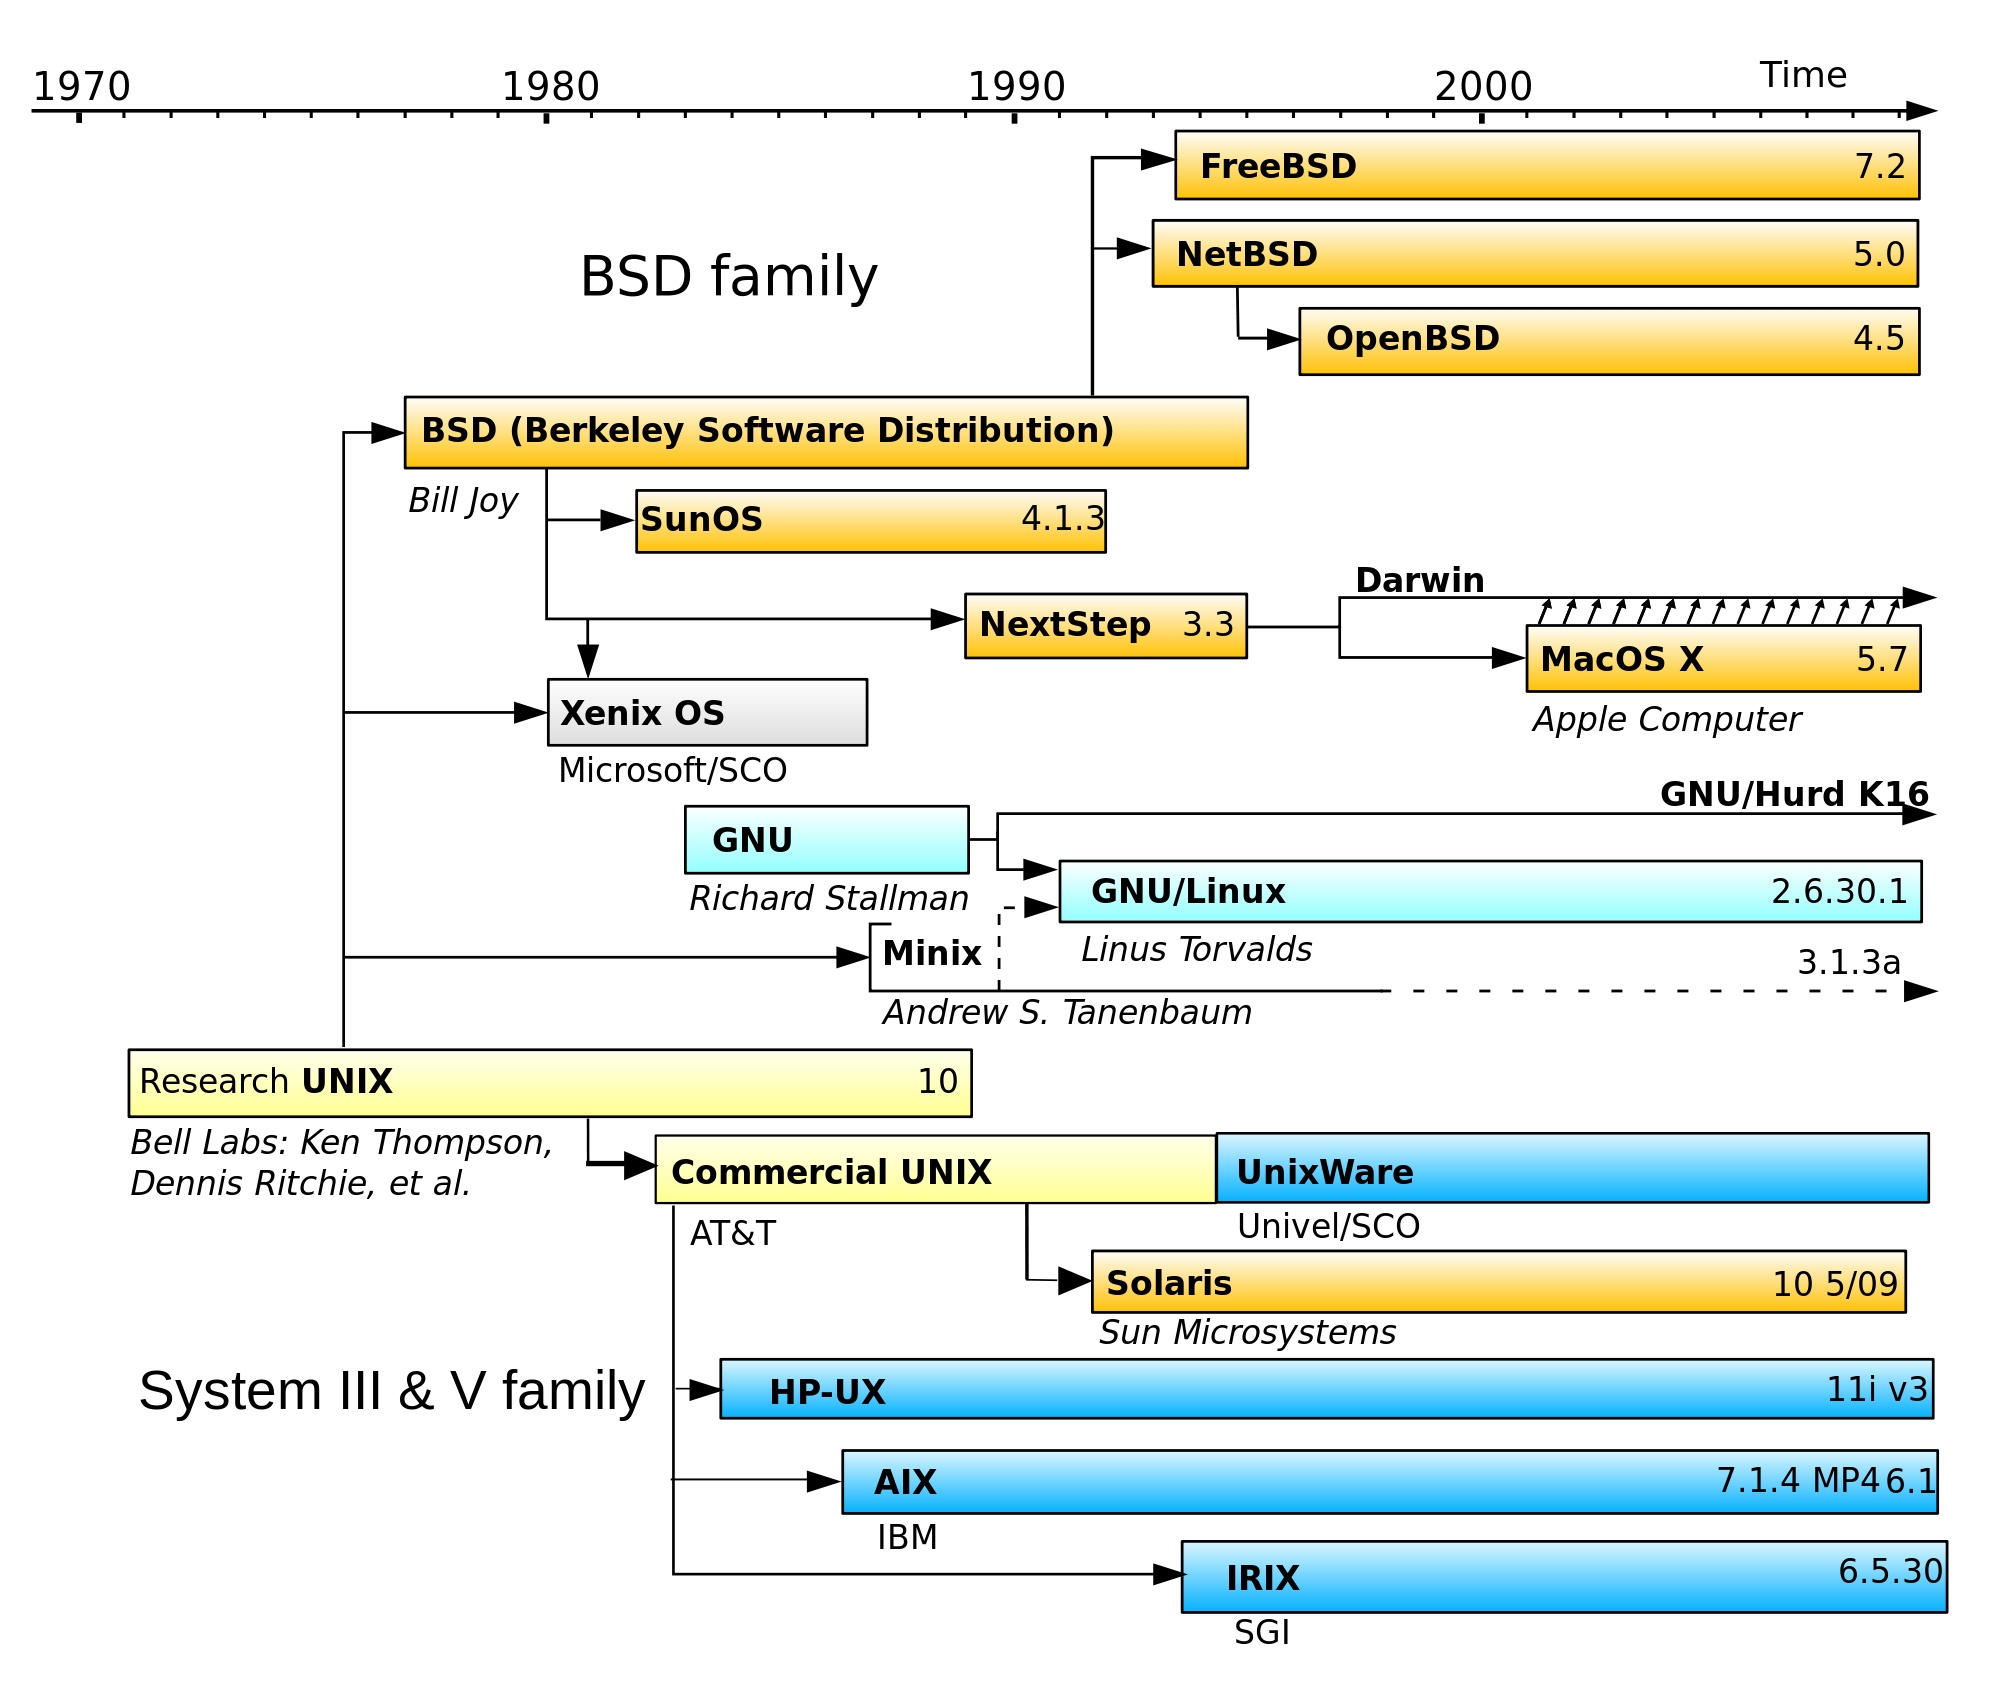
\includegraphics[width=0.75\textwidth]{./Unix_history}
  \end{center}
\end{frame}

\begin{frame}
  \frametitle{\small What is Linux?}
  \begin{itemize}
    \item Linux is an operating system that evolved from a kernel created by Linus Torvalds when he was a student at the University of Helsinki. 
    \item It's meant to be used as an alternative to other operating systems, Windows, Mac OS, MS-DOS, Solaris and others. 
    \item Linux is the most popular OS used in a Supercomputer\let\thefootnote\relax\footnote{\tiny \url{http://www.top500.org/statistics/list/}}
    \begin{center}
      \begin{tikzpicture}
        \node (tbl) {
          \begin{tabularx}{0.5\textwidth}{ccc}
            \arrayrulecolor{tigersgold}
            \textcolor{white}{\textbf{OS Family} }& \textcolor{white}{\textbf{Count}} &\textcolor{white}{\textbf {Share \%}}\\
            Linux \rule{0pt}{3.5ex} & 482 & 96.4 \\
            Unix & 11 & 2.2 \\
            Mixed & 4 & 0.8 \\
            Windows & 2 & 0.4 \\
            BSD Based & 1 & 0.2 \\
            [1.0ex]
        \end{tabularx}};
        \begin{pgfonlayer}{background}
          \draw[rounded corners,top color=blue!30!black,bottom color=blue!10!white,
            draw=tigerspurple!30] ($(tbl.north west)+(0.14,0)$)
          rectangle ($(tbl.north east)-(0.13,0.9)$);
          \draw[rounded corners,top color=green!5,bottom color=green!5,draw=green!5]
          ($(tbl.north east)-(0.13,0.6)$)
          rectangle ($(tbl.south west)+(0.13,0.2)$);
        \end{pgfonlayer}
      \end{tikzpicture}
    \end{center}
    \item If you are using a Supercomputer for your research, there is a 98\% probability that it will be based on a *nix OS.
  \end{itemize}
\end{frame}

\begin{frame}
  \frametitle{\small What is Linux?}
  \begin{itemize}
    \item Many software vendors release their own packaged Linux OS (kernel, applications) known as distribution
    \item Linux distribution = Linux kernel + GNU system utilities and libraries + Installation scripts + Management utilities etc.
    \begin{enumerate}
      {\footnotesize
        \item Debian, Ubuntu, Mint
        \item Red Hat, Fedora, CentOS
        \item Slackware, openSUSE, SLES, SLED
        \item Gentoo
      }
    \end{enumerate}
    \item Application packages on Linux can be installed from source or from customized packages
    \begin{enumerate}
      {\footnotesize
        \item deb: Debian based distros e.g. Debian, Ubuntu, Mint
        \item rpm: Red Hat based distros, Slackware based distros.
      }
    \end{enumerate}
    \item Linux distributions offer a variety of desktop environment.
    \begin{enumerate}
      {\scriptsize
        \item K Desktop Environment (KDE)
        \item GNOME 
        \item Xfce
        \item Lightweight X11 Desktop Environment (LXDE)
        \item Cinnamon
        \item MATE
      }
    \end{enumerate}
  \end{itemize}
\end{frame}

\begin{frame}{\small openSUSE KDE Desktop}
  \begin{center}
    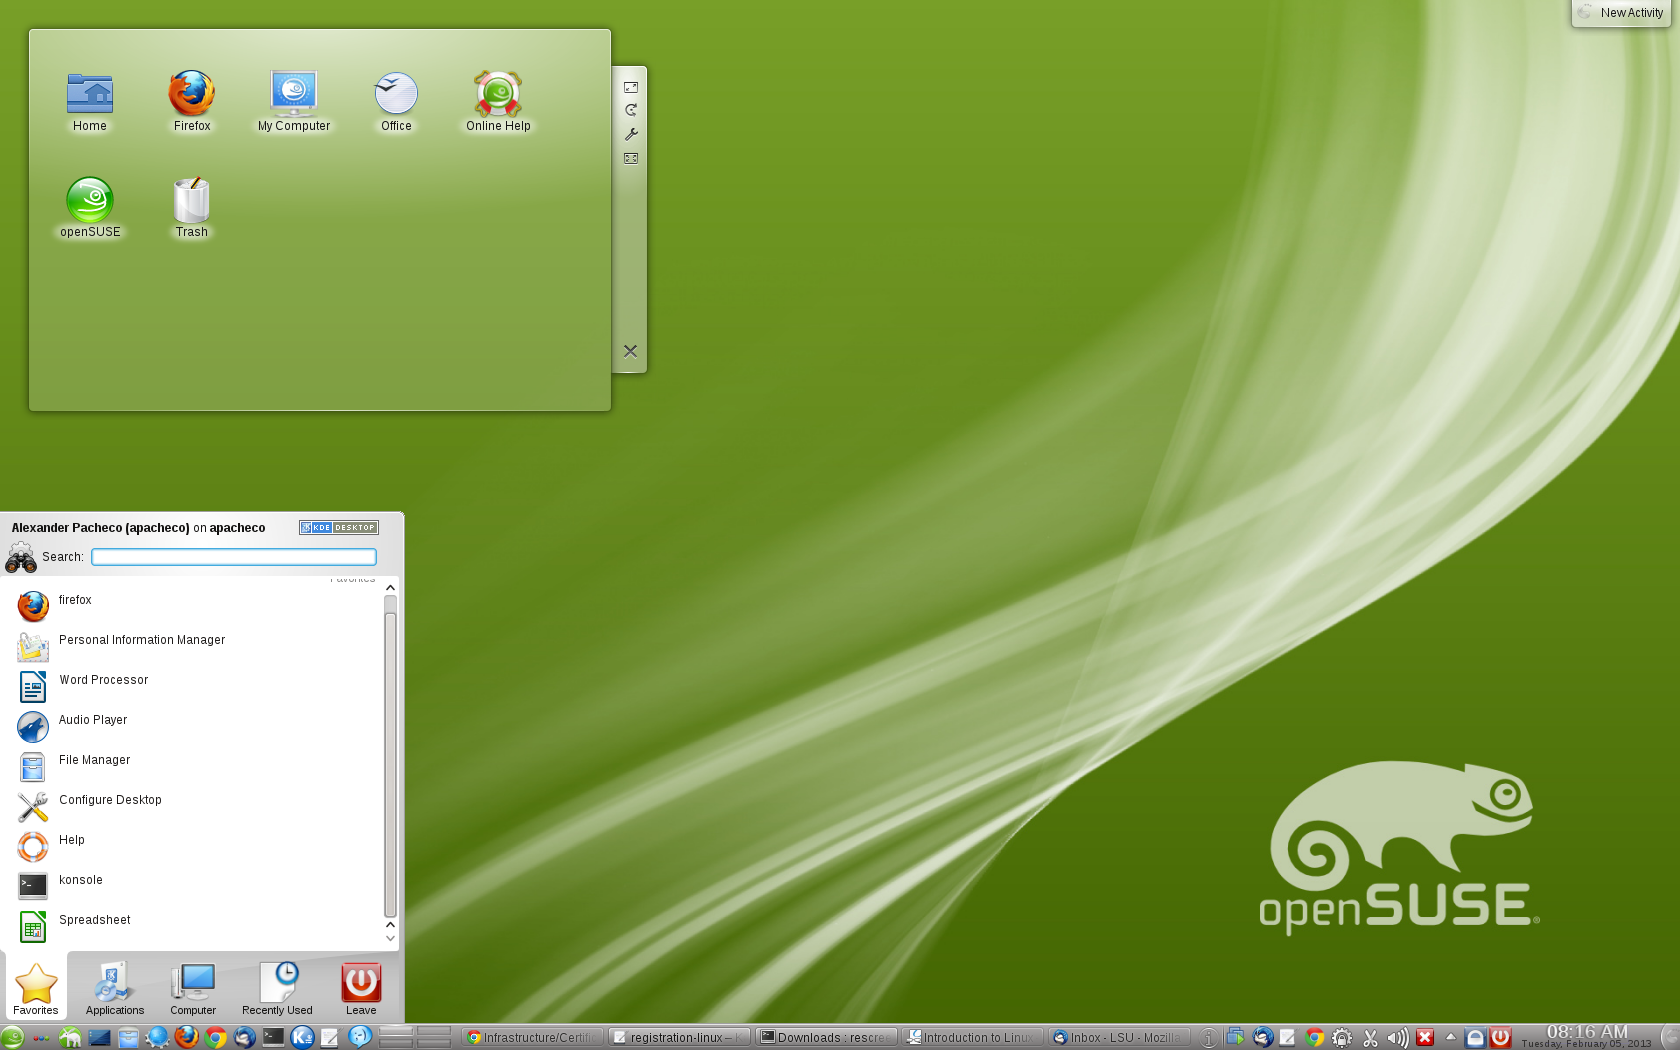
\includegraphics[width=\textwidth]{./opensuse}
  \end{center}
\end{frame}
\begin{frame}{\small CentOS GNOME Desktop}
  \begin{center}
    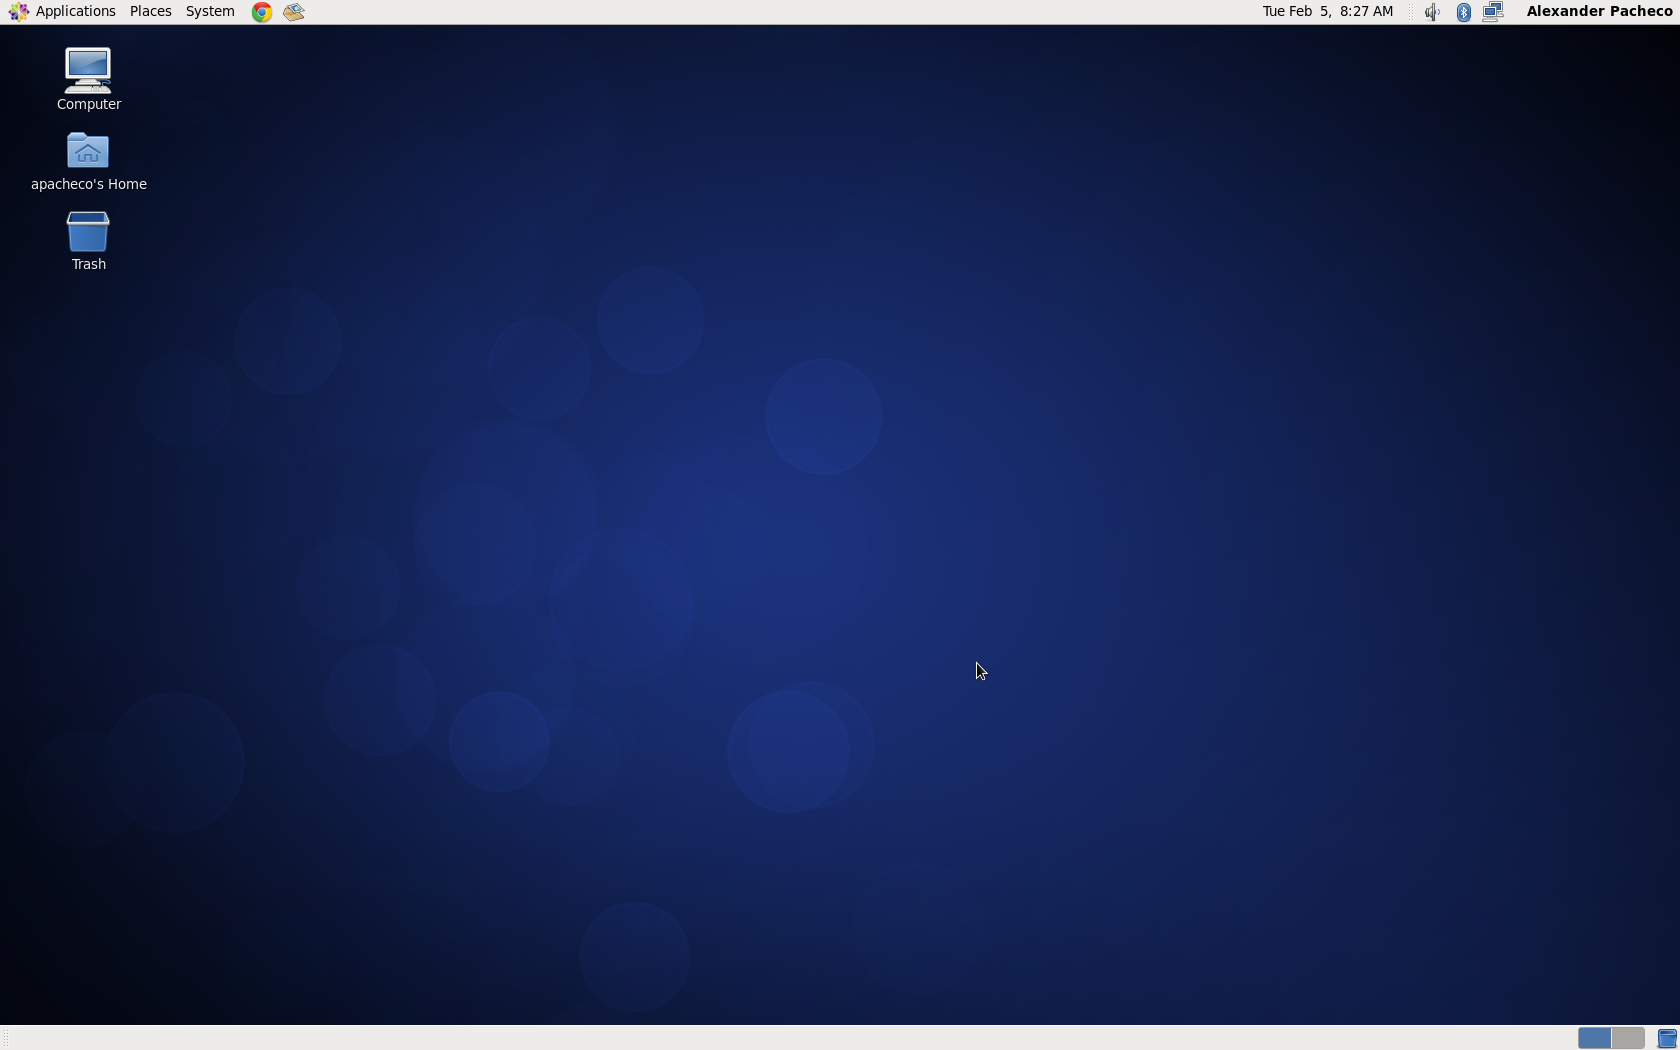
\includegraphics[width=\textwidth]{./CentOS6_3}
  \end{center}
\end{frame}
\begin{frame}{\small LXDE Desktop}
  \begin{center}
    
\includegraphics[width=0.9\textwidth]{./LXDE_desktop_full}
  \end{center}
\end{frame}
\begin{frame}{\small Debian MATE Desktop}
  \begin{center}
    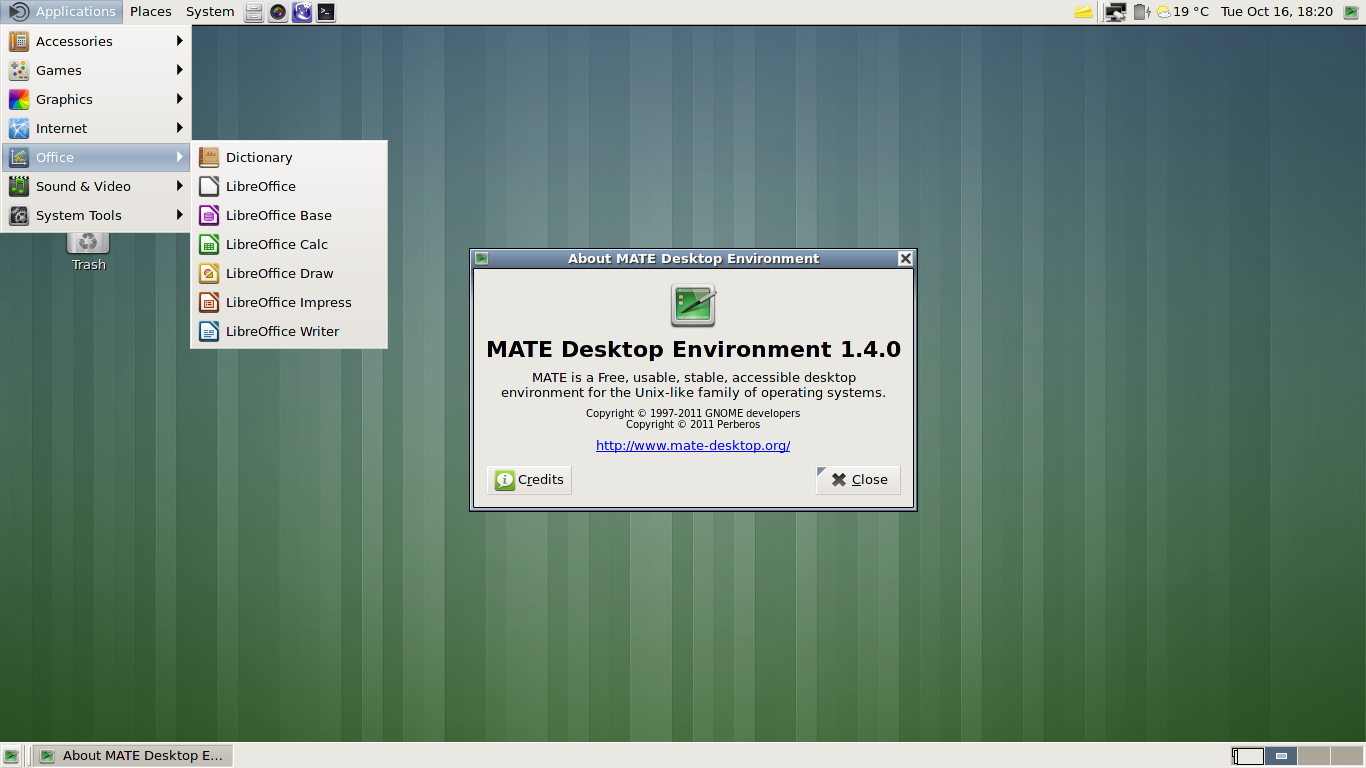
\includegraphics[width=\textwidth]{./Mate_DE_on_Debian}
  \end{center}
\end{frame}
\begin{frame}{\small Linux Mint Cinnamon Desktop}
  \begin{center}
    
\includegraphics[width=\textwidth]{./Cinnamon_Mint}
  \end{center}
\end{frame}


\begin{frame}
  \frametitle{\small What is Linux?}
  \begin{itemize}
    \item Linux distributions are tailored to different requirements such as
    \begin{enumerate}
      {\footnotesize
        \item Server
        \item Desktop
        \item Workstation
        \item Routers
        \item Embedded devices
        \item Mobile devices (Android is a Linux-based OS)
      }
    \end{enumerate}
    \item Almost any software that you use on windows has a roughly equivalent software on Linux, most often multiple equivalent software
    \item[e.g.] Microsoft Office equivalents are OpenOffice.org, LibreOffice, KOffice
    \item For complete list, visit \url{http://wiki.linuxquestions.org/wiki/Linux_software_equivalent_to_Windows_software}
    \item Linux offers you freedom, to choose your desktop environment, software.
  \end{itemize}
\end{frame}

\begin{frame}[fragile]
  \frametitle{\small Popularity of Linux Distributions}
  \begin{columns}
    \column{0.43\textwidth}
    \vspace{-0.2cm}
    \begin{itemize}
      \item \href{http://distrowatch.com/}{\color{blue}DistroWatch} provides news, popularity rankings, and other general information about:
      \begin{enumerate}
        {\scriptsize
          \item various Linux distributions,
          \item free software/open source Unix-like operating systems such as OpenSolaris, MINIX and BSD.
        }
      \end{enumerate}
      \item DistroWatch is NOT an indication of market-share or quality nor is it an indication of how many users but  it is clearly an indication of what users are looking at.
    \end{itemize}
    \column{0.57\textwidth}
    \vspace{-1cm}
    \begin{center}
      \begin{matrixtable}{1.2cm}{2.4cm}{1.2cm}{0.6cm}{
          \head{Rank}   & \head{Distribution} & \head{Hits} & \\
          1 & Mint      & 3614 & \up   \\
          2 & Mageia    & 2418 & \down \\
          3 & Ubuntu    & 1906 & \up   \\
          4 & Fedora    & 1558 & \up   \\
          5 & OpenSUSE  & 1349 & \down   \\
          6 & Debian    & 1345 & \up   \\
          7 & Arch      & 1211 & \down   \\
          8 & PCLinuxOS & 1186 & \up   \\
          9 & Snowlinux & 877  & \up   \\
          10& Zorin     & 861  & \const \\
        }
      \end{matrixtable}
    \end{center}
  \end{columns}
\end{frame}

\begin{frame}[allowframebreaks]
  \frametitle{\small Linux Components}
  \begin{itemize}
    \item Linux is made up of two (three) parts:
    \begin{enumerate}
      {\footnotesize
        \item Kernel 
        \item Shell 
        \item Applications/Programs 
        }
    \end{enumerate}
  \end{itemize}
  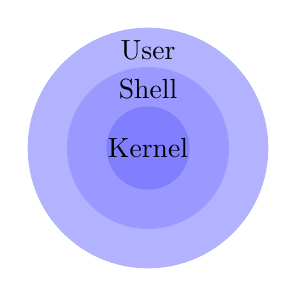
\begin{tikzpicture}
    \draw [fill=blue!30!white, ultra thick, blue!30!white] (3,0) circle (1.5);
    \draw [fill=blue!40!white, ultra thick, blue!40!white] (3,0) circle (1.0);
    \draw [fill=blue!50!white, ultra thick, blue!50!white] (3,0) circle (0.5);
    \node at (3,0) {Kernel};
    \node [above] at (3,.5) {Shell};
    \node [above] at (3,1) {User};
  \end{tikzpicture}
  
  \begin{eblock}{What is a kernel}
    \begin{itemize}
      \item The kernel is the main component of most computer operating systems
      \item It is a bridge between applications and the actual data processing done at the hardware level.
      \item The kernel's responsibilities include managing the system's resources (the communication between hardware and software components).
      \item provides the lowest-level abstraction layer for the resources (especially processors and I/O devices) that application software must control to perform its function.
      \item It typically makes these facilities available to application processes through inter-process communication mechanisms and system calls.
    \end{itemize}
  \end{eblock}
  \begin{eblock}{What is a SHELL}
    \begin{itemize}
      \item The command line interface is the primary interface to Linux/Unix operating systems.
      \item Shells are how command-line interfaces are implemented in Linux/Unix.
      \item Each shell has varying capabilities and features and the user should choose the shell that best suits their needs.
      \item The shell is simply an application running on top of the kernel and provides a powerful interface to the system.
    \end{itemize}
  \end{eblock}
\end{frame}

 
\begin{frame}
  \frametitle{\small Types of Shell}
  {\scriptsize
  \vspace{-0.25cm}
    \begin{itemize}
      \item[\texttt{sh}]: Bourne Shell
      \begin{enumerate}
        {\scriptsize
          \item[$\vardiamond$] Developed by Stephen Bourne at AT\&T Bell Labs
        }
      \end{enumerate}
      \item[\texttt{csh}]: C Shell
      \begin{enumerate}
        {\scriptsize
          \item[$\vardiamond$] Developed by Bill Joy at University of California, Berkeley
        }
      \end{enumerate}
      \item[\texttt{ksh}]: Korn Shell
      \begin{enumerate}
        {\scriptsize
          \item[$\vardiamond$] Developed by David Korn at AT\&T Bell Labs
          \item[$\vardiamond$] backward-compatible with the Bourne shell and includes many features of the C shell
        }
      \end{enumerate}
      \item[\texttt{bash}]: Bourne Again Shell
      \begin{enumerate}
        {\scriptsize
          \item[$\vardiamond$] Developed by Brian Fox for the GNU Project as a free software replacement for the Bourne shell (sh).
          \item[$\vardiamond$] Default Shell on Linux and Mac OSX
          \item[$\vardiamond$] The name is also descriptive of what it did, bashing together the features of sh, csh and ksh
        }
      \end{enumerate}
      \item[\texttt{tcsh}]: TENEX C Shell
      \begin{enumerate}
        {\scriptsize
          \item[$\vardiamond$] Developed by Ken Greer at Carnegie Mellon University 
          \item[$\vardiamond$] It is essentially the C shell with programmable command line completion, command-line editing, and a few other features.
        }
      \end{enumerate}
    \end{itemize}
  }
\end{frame}

\begin{frame}
  \frametitle{\small Shell Comparison}
  \begin{columns}
    \column{0.8\textwidth}
    \vspace{-1cm}
    \begin{center}
      \begin{tikzpicture}
        \node (tbl) {
          \begin{tabularx}{\textwidth}{cccccc}
            \arrayrulecolor{tigersgold}
            \textcolor{white}{\textbf{Software} }& \textcolor{white}{\textbf{sh}} &\textcolor{white}{\textbf {csh}} & \textcolor{white}{\textbf{ksh}} & \textcolor{white}{\textbf{bash}} & \textcolor{white}{\textbf{tcsh}} \\
            Programming Language\rule{0pt}{3.5ex} & \cmark & \cmark & \cmark & \cmark & \cmark \\
            Shell Variables & \cmark & \cmark & \cmark & \cmark & \cmark \\
            Command alias & \xmark & \cmark & \cmark & \cmark & \cmark \\
            Command history & \xmark & \cmark & \cmark & \cmark & \cmark \\
            Filename completion & \xmark & \smark & \smark & \cmark & \cmark \\
            Command line editing & \xmark & \xmark & \smark & \cmark & \cmark \\
            Job control & \xmark & \cmark & \cmark & \cmark & \cmark \\
            [1.0ex]
        \end{tabularx}};
        \begin{pgfonlayer}{background}
          \draw[rounded corners,top color=blue!30!black,bottom color=blue!10!white,
            draw=tigerspurple!30] ($(tbl.north west)+(0.14,0)$)
          rectangle ($(tbl.north east)-(0.13,0.9)$);
          %\draw[rounded corners,top color=tigersgold,bottom color=tigerspurple!20,
          %   middle color=tigerspurple!20,draw=tigerspurple!20] ($(tbl.south west)
          %   +(0.12,0.5)$) rectangle ($(tbl.south east)-(0.12,0)$);
          \draw[rounded corners,top color=green!5,bottom color=green!5,draw=green!5]
          ($(tbl.north east)-(0.13,0.6)$)
          rectangle ($(tbl.south west)+(0.13,0.2)$);
        \end{pgfonlayer}
      \end{tikzpicture}
      \begin{itemize}
        \item[\cmark]: Yes
        \item[\xmark]: No
        \item[\smark]: Yes, not set by default
        \item[Ref]: {\tiny\url{http://www.cis.rit.edu/class/simg211/unixintro/Shell.html}}
      \end{itemize}
    \end{center}
  \end{columns}
\end{frame}

\begin{frame}
  \frametitle{\small Files and Processes}
  \begin{itemize}
    \item Everything in Linux/UNIX is either a file or a process
    \item A File is a collection of data, created by users using text editors, running compilers, etc.
    \item Examples of Files:
    \begin{enumerate}
      {\footnotesize
        \item document such as collection of ascii text as in report, essay, etc. 
        \item program written in some high level programming language
        \item instructions comprehensible to machine but not a casual user such as executable, binary file
        \item directory containing information about its contents such as subdirectories or other files
      }
    \end{enumerate}
    \item A process is an executing program identified by a unique process identifier or PID.
  \end{itemize}
\end{frame}

\begin{frame}
  \frametitle{\small Directory Structure}
  \begin{columns}
    \column{1.1\textwidth}
    \vspace{-0.5cm}
  \begin{itemize}
    \item All files are arranged in a hierarchial structure, like an inverted tree.
    \item The top of the hierarchy is traditionally called \textbf{root} (written as a slash / )
  \end{itemize}
\tikzstyle{every node}=[draw=black,thick,anchor=west]
\tikzstyle{selected}=[draw=red,fill=red!30]
\tikzstyle{optional}=[dashed,fill=gray!50]
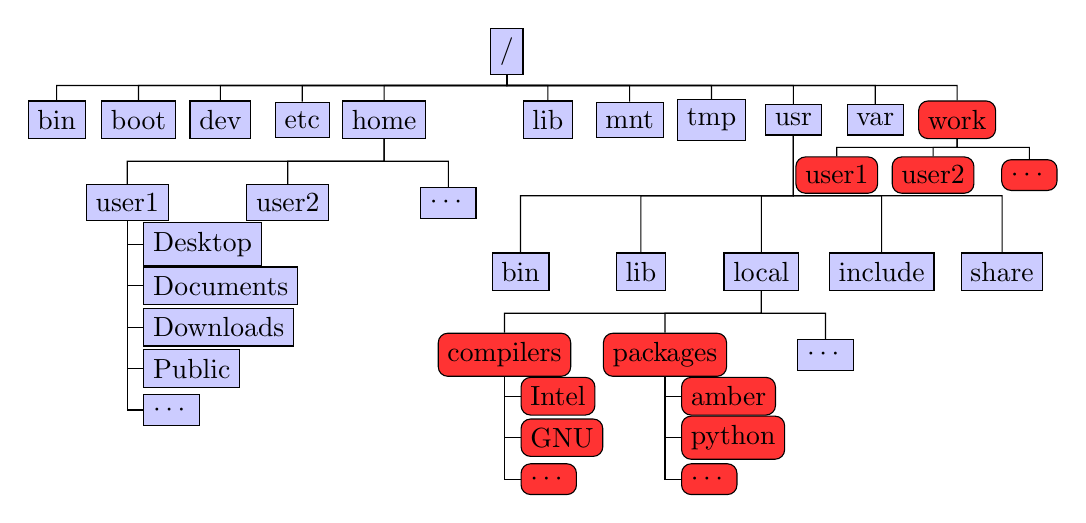
\begin{tikzpicture}[%
  linux/.style={rectangle,draw,fill=blue!20},
  hpc/.style={rectangle,draw,fill=red!80,rounded corners=.8ex},
  grandchild/.style={grow=down,xshift=1em,anchor=west,
    edge from parent path={(\tikzparentnode.south) |- (\tikzchildnode.west)}},
  first/.style={level distance=12ex,sibling distance=10em,xshift=-6em},
  second/.style={level distance=8ex,sibling distance=6em,xshift=-1.5em},
  third/.style={level distance=22ex,sibling distance=7.5em,xshift=-2em},
  fourth/.style={level distance=6ex},
  fifth/.style={level distance=12ex},
  sixth/.style={level distance=18ex},
  seventh/.style={level distance=24ex},
  eighth/.style={level distance=30ex},
  level 1/.style={sibling distance=5.1em},
  scale=0.58]
    % Parents
    \coordinate
    child[grow=down,level distance=0ex]{node[linux]{ / }}
    [edge from parent fork down]
    % Children and grandchildren
    child {node[linux] {bin}}
    child {node[linux] {boot}}
    child {node[linux] {dev}}
    child {node[linux] {etc}}
    child {node[linux] {home}
      child [first] {node[linux] {user1}
          child[grandchild,fourth] {node[linux] {Desktop}}
          child[grandchild,fifth] {node[linux] {Documents}}
          child[grandchild,sixth] {node[linux] {Downloads}}
          child[grandchild,seventh] {node[linux] {Public}}
          child[grandchild,eighth] {node[linux] {$\cdots$}}
       }
      child [first] {node[linux] {user2}
       }
      child [first] {node[linux] {$\cdots$}}
    }
    child [missing] {}
    child {node[linux] {lib}}
    child {node[linux] {mnt}}
    child {node[linux] {tmp}}
    child {node[linux] {usr}
      child [third] {node[linux] {bin}}
      child [third] {node[linux] {lib}}
      child [third] {node[linux] {local}
        child [first] {node[hpc] {compilers}
          child [grandchild,fourth] {node[hpc] {Intel}}
          child [grandchild,fifth] {node[hpc] {GNU}}
          child [grandchild,sixth] {node[hpc] {$\cdots$}}
        }
        child [first] {node[hpc] {packages}
          child [grandchild,fourth] {node[hpc] {amber}}
          child [grandchild,fifth] {node[hpc] {python}}
          child [grandchild,sixth] {node[hpc] {$\cdots$}}
        }
        child [first] {node[linux] {$\cdots$}}
      }
      child [third] {node[linux] {include}}
      child [third] {node[linux] {share}}
    }
    child {node[linux] {var}}
    child {node[hpc] {work}
      child [second] {node[hpc] {user1}}
      child [second] {node[hpc] {user2}}
      child [second] {node[hpc] {$\cdots$}}
    };
\end{tikzpicture}
\end{columns}
\end{frame}

\begin{frame}
  \frametitle{\small Important Directories}
  \begin{description}
    \item[/bin:] contains files that are essential for system operation, available for use by all users.
    \item[/lib,/lib64:] contains libraries that are essential for system operation, available for use by all users.
    \item[/var:] used to store files which change frequently (system level not user level)
    \item[/etc:] contains various system configurations
    \item[/dev:] contains various devices such as hard disk, CD-ROM drive etc
    \item[/sbin:] same as bin but only accessible by \textbf{root}
    \item[/tmp:] temporary file storage
    \item[/boot:] contains bootable kernel and bootloader
    \item[/usr:] contains user documentations, binaries, libraries etc
    \item[/home:] contains home directories of all users. This is the directory where you are at when you login to a Linux/UNIX system.
  \end{description}
  \begin{itemize}
    \item Installing your own OS: /bin,/lib\{64\},/etc,/dev and /sbin must be on the same partition.
  \end{itemize}
\end{frame}

\begin{frame}[fragile]
  \frametitle{\small }
  \begin{itemize}
    \item UNIX like OS's are designed for multi user environments i.e. multiple users can exist on the system.
    \item Special user called \textbf{root} is the administrator and has access to all files in the system.
    \item In *nix, users are organized into groups.
    \item Each user is in alteast one group.
    \item[$\bigstar$] On LONI systems, you are in one of the following groups: \Verbblue{lsuusers}, \Verbblue{latechusers}, \Verbblue{unousers}, \Verbblue{ullusers}, \Verbblue{sususers}, \Verbblue{tulaneusers}, \Verbblue{loni} or \Verbblue{xavierusers}
    \item Due to software licensing, you cannot be in more than one of the above groups.
    \item Group membership makes it easier to share files with members of your group or in the case of LONI systems, with researchers at your university.
    \item[]Type \Verbgreen{groups{\Enter}} to find your group membership.
    \item All files are \textit{case sensitive},
    \item[$\bigstar$] myfile.txt, Myfile.txt and myfile.TXT are three different files and can exist in the same directory simultaneously.
  \end{itemize}
\end{frame}

\begin{frame}
  \frametitle{\small Relative \& Absolute Path}
  \begin{itemize}
    \item \textit{Path} means a position in the directory tree.
    \item You can use either the \textit{relative path} or \textit{absolute path}
    \item In \textit{relative path} expression
    \begin{itemize}
      {\footnotesize
        \item . (one dot or period) is the current working directory
        \item .. (two dots or periods) is one directory up
        \item You can combine . and .. to navigate the file system hierarchy.
        \item the path is not defined uniquely and does depend on the current path.
        \item \texttt{../../tmp} is unique only if your current working directory is your home directory.
      }
    \end{itemize}
    \item In \textit{absolute path} expression 
    \begin{itemize}
      {\footnotesize
        \item the path is defined uniquely and does not depend on the current path
        \item \texttt{/tmp} is unique since /tmp is the \textit{abolute path}
      }
    \end{itemize}
  \end{itemize}
\end{frame}

\section{Variables}
\begin{frame}[fragile,allowframebreaks]
  \frametitle{\small Variables}
  \begin{itemize}
    \item *nix also permits the use of variables, similar to any programming language such as C, C++, Fortran etc
    \item A variable is a named object that contains data used by one or more applications. 
    \item There are two types of variables, Environment and User Defined and can contain  a number, character or a string of characters.
    \item Environment Variables provides a simple way to share configuration settings between multiple applications and processes in Linux.
    \item By Convention, enviromental variables are often named using all uppercase letters
    \item[e.g.] \Verbgreen{PATH, LD\_LIBRARY\_PATH, LD\_INCLUDE\_PATH, TEXINPUTS,} etc
    \item To reference a variable (environment or user defined) prepend \$ to the name of the variable
    \item[e.g.] \Verbgreen{\$PATH, \$LD\_LIBRARY\_PATH}
    \framebreak
%  \end{itemize}
%\end{frame}
%
%\begin{frame}[allowframebreaks]
%  \frametitle{\small Environment Variable}
%  \begin{itemize}
    \item The command \Verbgreen{printenv} list the current environmental variables.
    \item[$\bigstar$] {Type \Verbgreen{printenv} on your command prompt to list all environment variables in your current session.}
    \item The command \Verbgreen{env} is used to either print a list of environment variables or run another utility in an altered environment without having to modify the currently existing environment.
    \item[$\bigstar$] {Type \Verbgreen{env SHELL=/bin/tcsh xterm} to start an xterm session in tcsh}
    \item[$\vardiamond$] {To execute the above command successfully, you need to be in GUI mode on the virtual OS or logged into a remote systems with X-Forwarding enabled.}
  \end{itemize}
  \framebreak
  \begin{description}
    \item[PATH:] A list of directory paths.
    \item[HOME:] indicate where a user's home directory is located in the file system.
    \item[PWD:] contains path to current working directory.
    \item[OLDPWD:] contains path to previous working directory.
    \item[TERM:] specifies the type of computer terminal or terminal emulator being used
    \item[SHELL:] contains name of the running, interactive shell.
    \item[PS1:] default command prompt
    \item[PS2:] secondary command prompt
    \item[LD\_LIBRARY\_PATH:] colon-separated set of directories where libraries should be searched for first
    \item[HOSTNAME:] The systems host name
    \item[USER:] Current logged in user's name
    \item[DISPLAY:] Network name of the X11 display to connect to, if available.
%    \item[LD\_INCLUDE\_PATH:] 
  \end{description}
  \framebreak
  \begin{itemize}
    \item You can edit the environment variables.
    \item Command to do this depends on the shell
    \item[$\bigstar$] To add your bin directory to the \Verbgreen{PATH} variable
    \item[] \Verbpurple{sh/ksh/bash}: \Verbgreen{export PATH=\$\{HOME\}/bin:\$\{PATH\}}
    \item[] \Verbpurple{csh/tcsh}: \Verbgreen{setenv PATH \$\{HOME\}/bin:\$\{PATH\}}
    \item[$\bigstar$] Note the syntax for the above commands
    \item[$\bigstar$] \Verbpurple{sh/ksh/bash:} {no spaces except between \Verbgreen{export} and \Verbgreen{PATH}}
    \item[$\bigstar$] \Verbpurple{csh,tcsh:} {no = sign, just a space between \Verbgreen{PATH} and the absolute path}
    \item[$\bigstar$] \Verbpurple{all shells:} {colon(:) to separate different paths and the variable that is appended to}
    \item \textbf{Yes, the order matters.} If you have a customized version of a software say perl in your home directory, if you append the perl path to \Verbgreen{PATH} at the end, your program will use the system wide perl not your locally installed version.
      \framebreak
    \item Rules for Variable Names
    \begin{enumerate}
      \fontsize{8}{10}\selectfont{
        \item Variable names must start with a letter or underscore
        \item Number can be used anywhere else
        \item DO NOT USE special characters such as \texttt{@, \#, \%, \$}
        \item Case sensitive
        \item Examples
        \begin{itemize}
          \fontsize{8}{10}\selectfont{
          \item Allowed: VARIABLE, VAR1234able, var\_name, \_VAR
          \item Not Allowed: 1VARIABLE, \%NAME, \$myvar, VAR@NAME 
          }
        \end{itemize}
      }
    \end{enumerate}
    \item Assigning value to a variable
    \begin{center}
      \begin{tikzpicture}
        \node (tbl) {
          \begin{tabularx}{0.8\textwidth}{ccc}
            \arrayrulecolor{tigersgold}
            \textcolor{white}{\textbf{Type} }& \textcolor{white}{\textbf{sh,ksh,bash}} &\textcolor{white}{\textbf {csh,tcsh}}\\
            Shell \rule{0pt}{3.5ex} & name=value & set name = value \\
            Environment & export name=value & setenv name value \\
            [1.0ex]
        \end{tabularx}};
        \begin{pgfonlayer}{background}
          \draw[rounded corners,top color=blue!30!black,bottom color=blue!10!white,
            draw=tigerspurple!30] ($(tbl.north west)+(0.14,0)$)
          rectangle ($(tbl.north east)-(0.13,0.9)$);
          \draw[rounded corners,top color=green!5,bottom color=green!5,draw=green!5]
          ($(tbl.north east)-(0.13,0.6)$)
          rectangle ($(tbl.south west)+(0.13,0.2)$);
        \end{pgfonlayer}
      \end{tikzpicture}
    \end{center}
    \item \Verbpurple{sh,ksh,bash} THERE IS NO SPACE ON EITHER SIDE OF =
    \item \Verbpurple{csh,tcsh} space on either side of = is allowed for the \Verbgreen{set} command
    \item \Verbpurple{csh,tcsh} There is no = in the \Verbgreen{setenv} command
  \end{itemize}
  \framebreak
  \begin{eblock}{Exercise}
    \begin{itemize}
      \item Create two shell variables containing
      \begin{enumerate}
        {\footnotesize
          \item your name
          \item[e.g.] MYNAME=Alex
          \item a standard greeting
          \item[e.g.] Greet=Hello
        }
      \end{enumerate}
      \item We'll make use of this variables in a few slides when we learn some basic commands.
    \end{itemize}
  \end{eblock}
\end{frame}

\section{Basic Commands}
\begin{frame}[fragile]
  \frametitle{\small Basic Commands}
  \begin{eblock}{What is a command and how do you use it?}
    \begin{itemize}
      \item \textbf{command} is a directive to a computer program acting as an interpreter of some kind, in order to perform a specific task.
      \item \textbf{command prompt} (or just \textbf{prompt}) is a sequence of (one or more) characters used in a command-line interface to indicate readiness to accept commands.
      \item Its intent is to literally prompt the user to take action. 
      \item A prompt usually ends with one of the characters \$, \%, \#, :, > and often includes other information, such as the path of the current working directory.
      \item[$\bigstar$] Virtual Image: \Verb[formatcom=\color{indigo},fontseries=b,commandchars=\\\{\}]|[user@localhost ~]\$|
%      \item[$\bigstar$] QueenBee: \texttt{[apacheco@qb4 $\sim$]\$}
      \item[$\bigstar$] Mac OSX in \Verbpurple{tcsh}: \Verb[formatcom=\color{indigo},fontseries=b,commandchars=\\\{\}]|[c8-bc-c8-ee-b8-9e:~] apacheco\%|
      \item Each \textbf{command} consists of three parts: name, options, arguments
      \item[] \Verb[formatcom=\color{indigo},fontseries=b,commandchars=\\\{\}]|[user@localhost ~]\$ command options arguments|
    \end{itemize}
  \end{eblock}
\end{frame}

\begin{frame}[fragile]{How to get more information with Linux}
  \begin{itemize}
    \item \Verbgreen{man} shows the manual for a command or program.
    \item The manual is a file that shows you how to use the command and list the different options for the command in question.
    \item Usage: \Verbgreen{man [command]}
    \item Example: \Verbgreen{man ls{\Enter}}
    \item \Verbgreen{apropos} shows you all of the man pages that may shed some light on a certain command.
    \item Usage: \Verbgreen{appropos [keyword]}
    \item Example: \Verbgreen{appropos editor{\Enter}}
  \end{itemize}
% leave space for info command
\end{frame}



\begin{frame}[fragile,allowframebreaks]
  \frametitle{\small Input \& Output Commands}
  \begin{itemize}
    \item The basis I/O statements are \Verbgreen{echo} for displaying output to screen and \Verbgreen{read} for reading input from screen/keyboard/prompt
    \item The \Verbgreen{read} statement takes all characters typed until the \Verbgreen{{\Enter}} key is pressed and stores them into a variable.
    \item Usage: \Verbgreen{read <variable name>}
    \item Example: \Verbgreen{read name{\Enter}}
    \item[] \Verbblue[it]{Alex Pacheco{\Enter}}
    \item In the above example, the name that you enter in stored in the variable \Verbpurple{name}.
    \item[]
    \item The \Verbgreen{echo arguments} command will print \Verbpurple{arguments} to screen or standard output. 
    \item \Verbpurple{arguments} can be a (single or multiple) variable, string of characters or numbers.
      \framebreak
    \item Examples:
      \begin{enumerate}
        {\footnotesize
          \item \Verbgreen{echo \$LD\_LIBRARY\_PATH \$LD\_INCLUDE\_PATH{\Enter}}
          \item \Verbgreen{echo Welcome to HPC {\quad} Training{\Enter}}
        }
      \end{enumerate}
    \item By default, \Verbgreen{echo} eliminates redundant whitespace (multiple spaces and tabs) and replaces it with a single whitespace between arguments. 
    \item To include redundant whitespace, enclose the arguments within double quotes
    \item[e.g.] \Verbgreen{echo "Welcome to HPC{\quad\quad}Training"{\Enter}}
  \end{itemize}

  \begin{eblock}{Exercise}
    \begin{itemize}
      \item Print out the variable you created a few slides back
      \item[] \Verbgreen{echo \$MYNAME{\Enter}}
      \item[] \Verbgreen{echo \$Greet{\Enter}}
      \item Read a variable for greeting message
      \item[] \Verbgreen{read message{\Enter}}
      \item[] \Verbblue[it]{Welcome to HPC{\Enter}}
      \item Combine and print your name, the greeting and the message
      \item[] \Verbgreen{echo \$Greet \$MYNAME \$message{\Enter}}
      \item What is the output of the following command?
      \item[] \Verbgreen{echo \$Greet \$MYNAME, \$message Training{\Enter}}
    \end{itemize}
  \end{eblock}
\end{frame}

\begin{frame}[fragile]{Commands: pwd \& cd}
  \begin{itemize}
    \item \Verbgreen{pwd} command prints the current working directory.
    \item Usage: \Verbgreen{pwd}
    \item Example: \Verbgreen{pwd{\Enter}}
    \item[]{}
    \item \Verbgreen{cd} command allows one to change directory
    \item argument is the path (relative or absolute) of the directory you want to change to
    \item Usage: \Verbgreen{cd [destination]}
    \item Example: \Verbgreen{cd /tmp{\Enter}}
    \item The default destination directory is your home directory.
    \item i.e. If you type \Verbgreen{cd{\Enter}}, you will end up in your home directory.
    \item If you want to go back to the previous directory, type \Verbgreen{cd - {\Enter}}
  \end{itemize}
\end{frame}

\begin{frame}[fragile]{\small Command: ls}
  \begin{itemize}
    \item \Verbgreen{ls} command lists the contents of a directory.
    \item Usage: \Verbgreen{ls <options> <path>}
    \item Example: \Verbgreen{ls{\Enter}}
    \item The current working directory is the default path.
    \item To list contents of another directory specify the path, relative or absolute
    \item Common options to the \Verbgreen{ls} command 
    \item[] \Verbgreen{-l}: show long listing format
    \item[] \Verbgreen{-a}: show hidden files
    \item[] \Verbgreen{-r}: reverse order while sorting
    \item[] \Verbgreen{-t}: show modification times
    \item[] \Verbgreen{-h}: use file sizes in SI units (bytes, kilobytes, megabytes etc ) default is bytes
  \end{itemize}
\end{frame}

\begin{frame}[fragile]{\small Command: alias}
  \begin{itemize}
    \item \Verbgreen{alias} is a command to create a shortcut to another command or name to execute a long string.
    \item Usage 
    \item[] \Verbpurple{bash/sh/ksh}: \Verbgreen{alias <name>="<actual command>"}
    \item[] \Verbpurple{csh/tcsh}: \Verbgreen{alias <name> "<actual command>"}
    \item Example: 
    \item[] \Verbpurple{bash/sh/ksh}: \Verbgreen{alias lla="ls -al"}
    \item[] \Verbpurple{csh/tcsh}: \Verbgreen{alias lls "ls -al"}
    \item The \Verbgreen{alias} command is very useful tool to create shortcuts to other commands and is most often used by paranoid users to prevent accidental deletion of files. 
    \item \Verbgreen{unalias} is a command to remove an alias.
    \item Usage: \Verbgreen{unalias <name>}
    \item Example: \Verbgreen{unalias lla} will remove the shortcut to \Verbgreen{ls -al}
  \end{itemize}
\end{frame}

\begin{frame}[fragile]{\small Command: mkdir}
  \begin{itemize}
    \item \Verbgreen{mkdir} is a command to create a directory
    \item Usage: \Verbgreen{mkdir <options> <directoryname>}
    \item Example: \Verbgreen{mkdir -p \$HOME/test/testagain{\Enter}}
    \item By default, the directory is created in the current directory or in a path relative to the current directory
    \item The \Verbgreen{-p} option will create intermediate directories if they do not exist.
    \item[e.g.] If the directory \Verbgreen{test} does not exist in \Verbgreen{\$HOME}, then 
    \item[] \Verbgreen{mkdir \$HOME/test/testagain} will fail. 
    \item[] The \Verbgreen{-p} option will create the \Verbgreen{test} directory within \Verbgreen{\$HOME} and then create \Verbgreen{testagain} within the newly created \Verbgreen{test} directory
  \end{itemize}
\end{frame}

\begin{frame}[fragile]{\small Command: cp}
  \begin{itemize}
    \item \Verbgreen{cp} is a command to copy a file or directory
    \item Usage: \Verbgreen{cp <options> <source(s)> <destination>}
    \item Example: \Verbgreen{cp \$HOME/.bashrc ../../tmp{\Enter}}
    \item Common options to \Verbgreen{cp} command:
    \item[] \Verbgreen{-r}: copy recursively, required when copying directories.
    \item[] \Verbgreen{-i}: prompt if file exists on destination and can be copied over.
    \item[] \Verbgreen{-p}: preserve file access times, ownership etc.
    \item If there are more than one source files, then the destination (i.e. last entry or file) must be a directory.
    \item If the source(s) is(are) a file(s) and the destination is a directory, then the file(s) will be copied into the directory
    \item[e.g.]\Verbgreen{cp file1 file2 dir1{\Enter}}
    \item[] \Verbgreen{dir1} will contain the files \Verbgreen{file1} and \Verbgreen{file2}
    \item[] If \Verbgreen{dir1} is a file, then the above command will fail
  \end{itemize}
\end{frame}

\begin{frame}[fragile]{\small Command: rm}
  \begin{itemize}
    \item \Verbgreen{rm} command removes or deletes a file or directory
    \item Usage: \Verbgreen{rm <options> <file or directory>}
    \item Example: \Verbgreen{rm \$HOME/tmpfile{\Enter}}
    \item Common options to \Verbgreen{rm} command:
    \item[] \Verbgreen{-r}: remove recursively, required when copying directories.
    \item[] \Verbgreen{-i}: prompt if file really needs to be deleted
    \item[] \Verbgreen{-f}: force remove overrides the \Verbgreen{-i} option
    \item {\color{red}{\large\textsc{be careful while using the }\textbf{rm}\textsc{ command, deleted files cannot be recovered}}}
    \item To be on the safe side, create an \Verbgreen{alias} to the \Verbgreen{rm} command and only use the \Verbgreen{-f} option only if you are sure you want to delete the file or directory
    \item[] \Verbpurple{sh/ksh/bash}: \Verbgreen{alias rm="rm -i"}
    \item[] \Verbpurple{csh/tcsh}   : \Verbgreen{alias rm 'rm -i'}
    \item delete empty directories using the \Verbgreen{rmdir} command.
  \end{itemize}
\end{frame}

\begin{frame}[fragile]{\small Command: mv}
  \begin{itemize}
    \item \Verbgreen{mv} command moves or renames a file or directory
    \item Usage: \Verbgreen{mv <options> <source> <destination>}
    \item Example: \Verbgreen{mv test test1}
    \item If there are more than one source file, then the last file is the destination and must be a directory.
    \item Use the \Verbgreen{-i} option to prompt if a file or directory will be overwritten.
    \item If the source(s) is(are) a file(s) and the destination is a directory, then the file(s) will be copied into the directory.
    \item[e.g.]\Verbgreen{mv file1 file2 dir1{\Enter}}
    \item[] \Verbgreen{dir1} will contain the files \Verbgreen{file1} and \Verbgreen{file2}
    \item[] If \Verbgreen{dir1} is a file, then the above command will fail
  \end{itemize}
\end{frame}

\begin{frame}[fragile]{\small Pager Commands}
  \begin{itemize}
    \item To display a file to screen, *nix provides three commands at your disposal
    \item \Verbgreen{cat}: Show contents of a file.
    \item \Verbgreen{more}: Display contents one page at a time.
    \item \Verbgreen{less}: Display contents one page at a time but allow forward/backward scrolling
    \item[] \texttt{less > more} or \texttt{less is more, more or less}
    \item Usage: \Verbgreen{cat/more/less <options> <filename>}
    \item Example: \Verbgreen{cat .bashrc}
    \item To scroll forward in \Verbgreen{more} or \Verbgreen{less}, use the space bar, \texttt{CNTRL-f/d} or "Page Down" key.
    \item To scroll backwards in \Verbgreen{less} use \texttt{CNTRL-b/u} or "Page Up".
    \item A rarely used command, \Verbgreen{tac} does the opposite of \Verbgreen{cat} i.e. show contents of a file in reverse.
  \end{itemize}
\end{frame}

\begin{frame}[fragile,allowframebreaks]{\small Other Commands}
  \begin{itemize}
    \item[passwd:] change password (\alert{does not work on LSU HPC and LONI systems})
    \item[chsh:] change default shell (\alert{does not work on LSU HPC and LONI systems})
    \item[df:] report disk space usage by filesystem
    \item[du:] estimate file space usage - space used under a particular directory or files on a file system.
    \item[sudo:] run command as root (\alert{only if you have access})
    \item[mount:] mount file system (\alert{root only})
    \item[umount:] unmount file system (\alert{root only})
    \item[shutdown:] reboot or turn off machine (\alert{root only})
    \item[top:] Produces an ordered list of running processes
    \item[free:] Display amount of free and used memory in the system
    \item[file:] Determine file type
    \item[touch:] change file timestamps or create file if not present
    \item[date:] display or set date and time
    \item[find]: Find a file
    \item[] \Verbgreen{find /dir/to/search -name file-to-search}
%    \framebreak
%    \item[vi:] Edit a file using VI/VIM
%    \item[emacs:] Edit a file using Emacs
    \item[wc:] Count words, lines and characters in a file
    \item[] \Verbgreen{wc -l .bashrc}
    \item[grep:] Find patterns in a file
    \item[] \Verbgreen{grep alias .bashrc}
    \item[awk:] File processing and report generating
    \item[] \Verbgreen{awk '\{print \$1\}' file1}
    \item[sed:] Stream Editor
    \item[] \Verbgreen{sed 's/home/HOME/g' .bashrc}
    \item[set:] manipulate environment variables
    \item[] \Verbgreen{set -o emacs}
    \item[ln:] Link a file to another file
    \item[] \Verbgreen{ln -s file1 file2}
%    \item[\&:] run a job in background
%    \item[CNTRL-Z:] suspend a running job
%    \item[fg:] run a suspended job in foreground
%    \item[bg:] run a suspended job in background
%    \item[CNTRL-C:] Kill a running job
%    \item[jobs:] Show list of background jobs
    \item[wait:] wait until all backgrounded jobs have completed
%    \item[kill:] kill a running job, need to provide process id
    \item[which:] shows the full path of (shell) commands
%    \item[who:] show who is logged on
%    \item[whoami:] print effective userid
%    \item[finger:] user information lookup program
    \item[whatis:] display manual page descriptions
    \item[!name:] rerun previously executed command with the same arguments as before, \Verbgreen{name <args>}.
    \item[] Note that you do not always have to type the full command \Verbgreen{name}, just the minimum unique characters (no spaces) of \Verbgreen{name} need to be entered.
    \item[] If you had entered two commands \Verbgreen{name <args>} and \Verbgreen{nbme <args>}, then to rerun \Verbgreen{name}, use the command \Verbgreen{!na{\Enter}}. 
    \item[history:] display a list of last executed commands. Optional argument \Verbgreen{m} will list the last m commands. 
    \item[] All previously executed commands will be listed with a number \Verbblue{n}.
    \item[] To rerun a command from history which has number \Verbblue{n}, run the command \Verbgreen{!n{\Enter}} 
  \end{itemize}
  To learn more about these commands, type \Verbgreen{man {\em command}} on the command prompt
\end{frame}

\begin{frame}[fragile]{\small Filename Completion}
  \begin{itemize}
    \item Filename or Tab completion is a default feature in \Verbpurple{bash} and \Verbpurple{tcsh}.
    \item It allows to a user to automatically complete the file, directory or command name you are typing upto the next unique characters using the TAB key.
    \item Example: Your home directory contains directories \Verbindigo{Desktop}, \Verbindigo{Documents} and \Verbindigo{Downloads}.
    \item[] If you enter the command \Verbgreen{ls D{\Tab}}, you will be prompted with above the three directory names.
      \begin{lstlisting}[basicstyle=\color{indigo}\bfseries\scriptsize\ttfamily,escapechar=\%]
[user@localhost ~]%\$% ls D%\Tab%
Desktop/ Documents/ Downloads/
[user@localhost ~]%\$% ls Do%\Tab%
Documents/ Downloads/
[user@localhost ~]%\$% ls Do
      \end{lstlisting}
  \end{itemize}
\end{frame}

\begin{frame}[fragile]{\small How to Login to Remote Systems?}
  \begin{itemize}
    \item Most Linux/UNIX systems allow secure shell connections from other systems.
    \item[e.g.] You need to login using \Verbgreen{ssh} to the LSU HPC and LONI clusters.
    \item Usage: \Verbgreen{ssh <username>@<remote host>}
    \item Example: \Verbgreen{ssh apacheco@eric.loni.org}
    \item If your local machine is a UNIX-like system i.e. Linux, Mac OSX, BSD, AIX, Solaris etc and your username on the local machine is the same as that of the remote machine, then
    \item[] you can omit the \Verbgreen{<username>@} part of the argument.
    \item[] i.e. \Verbgreen{ssh <remote host>}
    \item If the remote machine is listening to ssh connections on a non default port (i.e. different from port 22) add \Verbgreen{-p <port number>} option
    \item[i.e.] \Verbgreen{ssh -p <port number> <user>@<remote host>}
    \item If you need to forward the display of an application from the remote system to your local system, add the \Verbgreen{-X} option to \Verbgreen{ssh}
    \item[] Example: \Verbgreen{ssh -X apacheco@eric.loni.org}
  \end{itemize}
\end{frame}

\begin{frame}[fragile,allowframebreaks]{\small File Transfer between two systems} 
  \begin{itemize}
    \item \Verbgreen{scp} is a command to copy files/directories between two *nix hosts over the SSH protocol.
    \item Usage: \Verbgreen{scp <options> <user>@<host>:/path/to/source/file {\textbackslash}}\\
    \Verbgreen{{\qquad}<user>@<host>:/path/to/destination/file/or/directory}
    \item[e.g.] You want to copy files between Eric Loni Cluster and your Linux Desktop/Laptop
    \item[] \Verbgreen{scp apacheco@eric.loni.org:/work/apacheco/somefile .}
    \item[] \Verbgreen{scp -r Public apacheco@eric.loni.org:/work/apacheco/}
    \item You can omit the \Verbgreen{<user>@} part of the argument if the username is the same on both systems.
    \item You can omit the \Verbgreen{<user>@<host>:} for your local machine.
    \item Common options are \Verbgreen{-r} and \Verbgreen{-p}, same meaning as \Verbgreen{cp}.
    \item add \Verbgreen{-P <port number>} option for non default ports.
      \framebreak
    \item \Verbgreen{rsync} is another utility that can be used to copy files locally and remotely.
    \item Usage: \Verbgreen{rsync <option> <source> <destination>}
    \item It is famous for its delta-transfer algorithm
    \item[i.e.] sending only the differences between  the  source  files and  the  existing  files in the destination.  
    \item Rsync is widely used for backups and mirroring and as an improved copy command for everyday use.
    \item Common options:
      {\scriptsize
      \item[] \Verbgreen{-a}: archive mode
      \item[] \Verbgreen{-r}: recurse into directories
      \item[] \Verbgreen{-v}: increase verbosity
      \item[] \Verbgreen{-z}: compress file data during the transfer
      \item[] \Verbgreen{-u}: skip files that are newer on the receiver
      \item[] \Verbgreen{-t}: preserve modification times
      \item[] \Verbgreen{-n}: dry-run, perform a trial run with no changes made
      }
      \item Example: \Verb[formatcom=\color{dkgreen},fontseries=b,commandchars=\\\{\}]|rsync -avtzu eric.loni.org:~/* .|
  \end{itemize}
\end{frame}

\begin{frame}[fragile,allowframebreaks]{\small Compressing and Archiving Files}
  \begin{itemize}
    \item Quite often you need to compress and uncompress files to reduce storage usage or bandwidth while transferring files.
    \item *nix systems have built-in utilities to compress/uncompress files
      \begin{columns}
        \column{0.4\textwidth}
        \begin{eblock}{Compress}
          \Verbgreen{gzip, zip, bzip2}\\
          \Verbgreen{gzip README{\Enter}}
        \end{eblock}
        \column{0.4\textwidth}
        \begin{eblock}{Uncompress}
          \Verbgreen{gunzip, unzip, bunzip2}\\
          \Verbgreen{gunzip README.gz{\Enter}}
        \end{eblock}
      \end{columns}
    \item Gzipped files have an extension \Verbpurple{.gz,.z} or \Verbpurple{.Z}
    \item zipped files have an extension \Verbpurple{.Zip} or \Verbpurple{.zip}
    \item Bzipped files have an extension \Verbpurple{.bz2, .bz}
    \item To compress/uncompress files recursively, use the \Verbgreen{-r} option.
    \item To overwrite files while compressing/uncompressing, use the \Verbgreen{-f} option.
      \framebreak
    \item *nix provides the \Verbgreen{tar} package to create and manipulate streaming archive of files.
    \item Usage: \Verbgreen{tar <options> <file> <patterns>}
    \item[] \Verbgreen{file} is the name of the tar archive file, usually with extension \Verbgreen{.tar}
    \item[] \Verbgreen{patterns} are pathnames for files/directories being archived
    \item Common options
    \item[] \Verbgreen{-c}: create an archive file
    \item[] \Verbgreen{-x}: extract to disk from archive
    \item[] \Verbgreen{-z}: filter the archive through gzip (adds/requires extension .gz)
    \item[] \Verbgreen{-j}: filter the archive through bzip2 (adds/requires extension .bz2)
    \item[] \Verbgreen{-t}: list contents of archive
    \item[] \Verbgreen{-v}: verbosely list files processed
    \item[e.g.] \Verbgreen{tar -cvzf myhome.tar.gz \$\{HOME\}/*}
    \item This becomes useful for creating a backup of your files and directories that you can store at some storage facility e.g. external disk
  \end{itemize}
\end{frame}

\section{Redirection}
\begin{frame}
  \frametitle{\small I/O Redirection}
  \begin{itemize}
    \item There are three file descriptors for I/O streams
    \begin{enumerate}
      {\footnotesize
        \item[STDIN]: Standard Input
        \item[STDOUT]: Standard Output
        \item[STDERR]: Standard Error
      }
    \end{enumerate}
    \item 1 represents STDOUT and 2 represents STDERR
    \item I/O redirection allows users to connect applications
    \begin{itemize}
      {\footnotesize
      \item[<]: connects a file to STDIN of an application
      \item[>]: connects STDOUT of an application to a file
      \item[> >]: connects STDOUT of an application by appending to a file
      \item[|]: connects the STDOUT of an application to STDIN of another application.
      }
    \end{itemize}
    \item Examples:
    \begin{enumerate}
      {\footnotesize
      \item write STDOUT to file: \Verbgreen{ls -l > ls-l.out }
      \item write STDERR to file: \Verbgreen{ls -l 2> ls-l.err }
      \item write STDOUT to STDERR: \Verbgreen{ls -l 1>\&2 }
      \item write STDERR to STDOUT: \Verbgreen{ls -l 2>\&1 }
      \item send STDOUT as STDIN: \Verbgreenp{ls -l | wc -l}
      }
    \end{enumerate}
  \end{itemize}
\end{frame}

\section{File Permissions}

\begin{frame}[fragile, allowframebreaks]
  \frametitle{\small File Permissions}
  \begin{itemize}
    \item Since *NIX OS's are designed for multi user environment, it is necessary to restrict access of files to other users on the system.
    \item In *NIX OS's, you have three types of file permissions
    \begin{enumerate}
      {\footnotesize
        \item read (r)
        \item write (w)
        \item execute (x)
      }
    \end{enumerate}
    \item for three types of users
    \begin{enumerate}
      {\footnotesize
        \item user (u)
        \item group (g)
        \item world (o) i.e. everyone else who has access to the system
      }
    \end{enumerate}
    \begin{Verbatim}[formatcom=\color{indigo},fontsize=\scriptsize]
[user@localhost ~]$ ls -l
total 44
drwxr-xr-x. 2 user user 4096 Jan 28  2013 Desktop
drwxr-xr-x. 2 user user 4096 Jan 28  2013 Documents
drwxr-xr-x. 2 user user 4096 Jan 28  2013 Downloads
-rwxr-xr-x. 1 user user   32 Sep 11 11:57 hello
drwxr-xr-x. 2 user user 4096 Jan 28  2013 Music
drwxr-xr-x. 2 user user 4096 Jan 28  2013 Pictures
drwxr-xr-x. 2 user user 4096 Jan 28  2013 Public
-rw-rw-r--. 1 user user 3047 Sep 11 11:48 README
drwxr-xr-x. 1 root root 4216 Jan 22 16:17 Shared
drwxr-xr-x. 2 user user 4096 Jan 28  2013 Templates
lrwxrwxrwx. 1 user user    5 Jan 23 08:17 test -> hello
drwxr-xr-x. 2 user user 4096 Jan 28  2013 Videos
[user@localhost ~]$ 
    \end{Verbatim}
    \item The first character signifies the type of the file
    \item[] \Verb[formatcom=\color{indigo}]|d| for directory
    \item[] \Verb[formatcom=\color{indigo}]|l| for symbolic link
    \item[] \Verb[formatcom=\color{indigo}]|-| for normal file
    \item The next three characters of first triad signifies what the owner can do
    \item The second triad signifies what group member can do
    \item The third triad signifies what everyone else can do
      \begin{gather*}
        d\underbrace{rwx}_{u}\overbrace{r-x}^g\underbrace{r-x}_o
      \end{gather*}
    \item Read carries a weight of 4
    \item Write carries a weight of 2
    \item Execute carries a weight of 1
    \item The weights are added to give a value of 7 (rwx), 6(rw), 5(rx) or 3(wx) permissions. 
    \item \Verbgreen{chmod} is a *NIX command to change permissions on a file
    \item[] Usage: \Verbgreen{chmod <option> <permissions> <file or directory name>}
    \item To give user rwx, group rx and world x permission, the command is
    \item[] \Verbgreen{chmod 751 filename}
    \framebreak
    \item Instead of using numerical permissions you can also use symbolic mode
    \item[u/g/o or a] user/group/world or all i.e. ugo
    \item[+/-] Add/remove permission
    \item[r/w/x] read/write/execute
    \item Give everyone execute permission: 
    \item[] \Verbgreen{chmod a+x hello.sh }
    \item[] \Verbgreen{chmod ugo+x hello.sh}
    \item Remove group and world read \& write permission: 
    \item[] \Verbgreen{chmod go-rw hello.sh}
    \item To change permissions recursively in a directory, use the option \Verbgreen{-R} (can also be used in the following two commands)
    \item[] \Verbgreen{chmod -R 755 \$\{HOME\}/*}
    \item[] What is the permission on \$\{HOME\}?
    \framebreak
    \item The \Verbgreen{chgrp} command is used to change the group ownership between two groups that you are a member of.
    \item[] Usage: \Verbgreen{chgrp <option> <new group> <file or directory name>}
    \item[e.g.] Suppose your default group on LSU HPC is \Verbblue{users} and your advisor requested sysadmins to create a group \Verbblue{abc} for collaborative research among say 10 researchers. 
    \item You can use the \Verbgreen{chgrp} command to change the ownership of your files from the \Verbblue{users} group to \Verbblue{abc} group.
    \item[] Example: \Verbgreen{chgrp -R abc collaborative-work-dir}
    \item The \Verbgreen{chown} command is used to  change the owner of a file.
    \item \Verbgreen{chown} can only be executed by the superuser, to prevent users simply changing ownership of files that aren't theirs to access. 
    \item[] Usage: \Verbgreen{chown <new owner>[:<group name>] <file or directory name>}
  \end{itemize}
\end{frame}

\section{Process Management}
\begin{frame}[fragile,allowframebreaks]{\small Processes and Jobs}
  \begin{itemize}
    \item A process is an executing program identified by a unique PID
    \item[$\bigstar$] To see information about your running processes and their PID and status,
    \item[] \Verbgreen{ps{\Enter}}
    \item A process may be in foreground, background or be suspended.
    \item Processes running in foreground, the command prompt is not returned until the current process has finished executing.
    \item If a job takes a long time to run, put the job in background in order to obtain the command prompt back to do some other useful work
    \item There are two ways to send a job into the background:
    \begin{enumerate}
      {\footnotesize
        \item Add an ampersand \Verbgreen{\&} to the end of your command to send it into background directly.
        \item[] \Verbblue{firefox \&{\Enter}}
        \item First suspend the job using \Verbblue{{\Ctrl}Z} and then type \Verbblue{bg} at the command prompt.
        \item If you type \Verbblue{fg} then the job will run in foreground and you will lose the command prompt.
      }
    \end{enumerate}
    \framebreak
    \item When a process is running, background or suspended, it will be entered onto a list along with a job number (not PID)
    \item[] \Verbgreen{jobs{\Enter}}
    \item To restart a suspended job in foreground or background, type
    \item[] \Verbgreen{fg \%jobnumber} where \Verbblue{jobnumber} is a number greater than 1, or,
    \item[] \Verbgreen{bg \%jobnumber} 
    \item To kill or terminate a process:
    \begin{enumerate}
      {\footnotesize
        \item Job running in foreground: enter \Verbblue{{\Ctrl}C}
        \item Job whose PID you know
        \item[] \Verbgreen{kill PID{\Enter}}
        \item Job whose \Verbblue{jobnumber} you know (from \Verbgreen{jobs} command)
        \item[] \Verbgreen{kill \%jobnumber{\Enter}}
      }
    \end{enumerate}
    \item The \Verbgreen{kill} command can take options specific to UNIX signals
    \item The most common option is \Verbgreen{-9} for the \Verbgreen{SIGKILL} signal
    \item \Verbgreen{pstree}: display a tree of processes
    \item \Verbgreen{pkill}: kill process by its name, user name, group name, terminal, UID, EUID, and GID.
  \end{itemize}
\end{frame}

\section{Editors}
\begin{frame}
  \frametitle{\small File Editing}
  \begin{itemize}
    \item The two most commonly used editors on Linux/Unix systems are:
    \begin{enumerate}
      \item \Verbgreen{vi} or \Verbgreen{vim} (vi improved)
      \item \Verbgreen{emacs}
    \end{enumerate}
    \item \Verbgreen{vi/vim} is installed by default on Linux/Unix systems and has only a command line interface (CLI).
    \item \Verbgreen{emacs} has both a CLI and a graphical user interface (GUI).
    \item[$\vardiamond$] If \Verbgreen{emacs} GUI is installed then use \Verbgreen{emacs -nw} to open file in console.
    \item Other editors that you may come across on *nix systems
    \item[] \Verbgreen{kate}: {default editor for KDE.}
    \item[] \Verbgreen{gedit}: {default text editor for GNOME desktop environment.}
    \item[] \Verbgreen{gvim}: {GUI version of }\Verbgreen{vim}
    \item[] \Verbgreen{pico}: {console based plain text editor }
    \item[] \Verbgreen{nano}: {GNU.org clone of }\Verbgreen{pico}
    \item[] \Verbgreen{kwrite}: {editor by KDE.}
  \end{itemize}
\end{frame}

\begin{frame}[allowframebreaks]
  \frametitle{\small Editor Cheatsheets}
% Page 1
  \begin{itemize}
    \item \textbf{\color{dkgreen}vi/vim} and \textbf{\color{dkgreen}emacs} are the two most popular *nix file editors.
    \item Which one to use is up to you.
    \item \textbf{\color{dkgreen}vi/vim} has two modes:
    \begin{enumerate}
      {\scriptsize
        \item Editing mode
        \item Command mode
      }
    \end{enumerate}
    \item \textbf{\color{dkgreen}emacs} has only one mode as in any editor that you use.
  \end{itemize}
  {\scriptsize
  \begin{columns}[t]
    \column{0.6\textwidth}
    \begin{eblock}{Insert/Appending Text}
    \begin{itemize}
      \item insert at cursor 
      \item insert at beginning of line
      \item append after cursor
      \item append at end of line
      \item newline after cursor in insert mode
      \item newline before cursor in insert mode
      \item append at end of line
      \item exit insert mode
    \end{itemize}
    \end{eblock}
    \column{0.2\textwidth}
    \begin{eblock}{vi}
    \begin{itemize}
      \item \texttt{i}
      \item \texttt{I}
      \item \texttt{a}
      \item \texttt{A}
      \item \texttt{o}
      \item \texttt{O}
      \item \texttt{ea}
      \item \texttt{ESC}
    \end{itemize}
    \end{eblock}
  \end{columns}
  }
  \framebreak
% Page 2
  \vspace{-0.6cm}
  {\scriptsize
  \begin{columns}
    \column{0.4\textwidth}
    \begin{eblock}{Cursor Movement}
    \begin{itemize}
      \item move left 
      \item move down
      \item move up
      \item move right
      \item jump to beginning of line
      \item jump to end of line
      \item goto line \texttt{n}
      \item goto top of file
      \item goto end of file
      \item move one page up
      \item move one page down
    \end{itemize}
    \end{eblock}
    \column{0.2\textwidth}
    \begin{eblock}{vi}
    \begin{itemize}
      \item \texttt{h}
      \item \texttt{j}
      \item \texttt{k}
      \item \texttt{l}
      \item \texttt{\^}
      \item \texttt{\$}
      \item \texttt{nG}
      \item \texttt{1G}
      \item \texttt{G}
      \item \texttt{C-u}
      \item \texttt{C-d}
    \end{itemize}
    \end{eblock}
    \column{0.4\textwidth}
    \begin{eblock}{emacs}
    \begin{itemize}
      \item \texttt{C-b}
      \item \texttt{C-n}
      \item \texttt{C-p}
      \item \texttt{C-f}
      \item \texttt{C-a}
      \item \texttt{C-e}
      \item \texttt{M-x goto-line \enter\, n}
      \item \texttt{M-<}
      \item \texttt{M->}
      \item \texttt{M-v}
      \item \texttt{C-v}
    \end{itemize}
    \end{eblock}
  \end{columns}
  }
  \vspace{-0.1cm}
  \begin{columns}
    \column{0.6\textwidth}
    \begin{itemize}
      {\scriptsize
      \item[C]: Control Key
      \item[M]: Meta or ESCAPE (ESC) Key
      \item[{\enter}]: Enter Key
      }
    \end{itemize}
  \end{columns}
  \framebreak
% Page 3
  {\scriptsize
   \begin{columns}
    \column{0.5\textwidth}
     \vspace{-0.5cm}
    \begin{eblock}{File Manipulation}
    \begin{itemize}
      \item save file
      \item save file and exit
      \item quit
      \item quit without saving
      \item delete a line
      \item delete \texttt{\textit{n}} lines
      \item paste deleted line after cursor
      \item paste before cursor
      \item undo edit
      \item delete from cursor to end of line
      \item search forward for \textit{patt}
      \item search backward for \textit{patt}
      \item search again forward (backward)
    \end{itemize}
    \end{eblock}
    \column{0.25\textwidth}
     \vspace{-0.5cm}
    \begin{eblock}{vi}
    \begin{itemize}
      \item \texttt{:w}
      \item \texttt{:wq, ZZ}
      \item \texttt{:q}
      \item \texttt{:q!}
      \item \texttt{dd}
      \item \texttt{\textit{n}dd}
      \item \texttt{p}
      \item \texttt{P}
      \item \texttt{u}
      \item \texttt{D}
      \item \texttt{$\backslash$\textit{patt}}
      \item \texttt{?\textit{patt}}
      \item \texttt{n}
    \end{itemize}
    \end{eblock}
    \column{0.3\textwidth}
     \vspace{-0.5cm}
    \begin{eblock}{emacs}
    \begin{itemize}
      \item \texttt{C-x C-s}
      \item \texttt{}
      \item \texttt{C-x C-c}
      \item \texttt{}
      \item \texttt{C-a C-k}
      \item \texttt{C-a M-\textit{n} C-k}
      \item \texttt{C-y}
      \item
      \item \texttt{C-\_}
      \item \texttt{C-k}
      \item \texttt{C-s \textit{patt}}
      \item \texttt{C-r \textit{patt}}
      \item \texttt{C-s(r)}
    \end{itemize}
    \end{eblock}
  \end{columns}
  }
  \framebreak
% Page 4
  {\scriptsize
  \begin{columns}
    \column{0.4\textwidth}
     \vspace{-0.5cm}
    \begin{eblock}{File Manipulation (contd)}
    \begin{itemize}
      \item replace a character
      \item join next line to current
      \item change a line
      \item change a word
      \item change to end of line
      \item delete a character
      \item delete a word
      \item edit/open file \textit{file}
      \item insert file \textit{file}
      \item split window horizontally
      \item split window vertically
      \item switch windows
    \end{itemize}
    \end{eblock}
    \column{0.35\textwidth}
     \vspace{-0.5cm}
    \begin{eblock}{vi}
    \begin{itemize}
      \item \texttt{r}
      \item \texttt{J}
      \item \texttt{cc}
      \item \texttt{cw}
      \item \texttt{c\$}
      \item \texttt{x}
      \item \texttt{dw}
      \item \texttt{:e \texttt{file}}
      \item \texttt{:r \texttt{file}}
      \item \texttt{:split or C-ws}
      \item \texttt{:vsplit or C-wv}
      \item \texttt{C-ww}
    \end{itemize}
    \end{eblock}
    \column{0.3\textwidth}
     \vspace{-0.5cm}
    \begin{eblock}{emacs}
    \begin{itemize}
      \item 
      \item 
      \item 
      \item
      \item
      \item \texttt{C-d}
      \item \texttt{M-d}
      \item \texttt{C-x C-f \textit{file}}
      \item \texttt{C-x i \textit{file}}
      \item \texttt{C-x 2}
      \item \texttt{C-x 3}
      \item \texttt{C-x o}
    \end{itemize}
    \end{eblock}
  \end{columns}
  }
  \framebreak
% Page 5
  \begin{itemize}
    \item Do a google search for more detailed cheatsheets
    \item[\texttt{vi}] \url{https://www.google.com/search?q=vi+cheatsheet}
    \item[\texttt{emacs}] \url{https://www.google.com/search?q=emacs+cheatsheet}
  \end{itemize}
  \begin{bblock}{More on the \textbf{set -o} command}
    \begin{itemize}
      \item The \textbf{\color{dkgreen}set -o} command can be used to change the command line editor mode among other things (Do \textbf{\color{dkgreen}man set\Enter} to find out more)
      \begin{enumerate}
        \item \textbf{\color{dkgreen}set -o emacs}: emacs style in-line editor for command entry, this is the default
        \item \textbf{\color{dkgreen}set -o vi}: vi style in-line editor for command entry.
      \end{enumerate}
    \end{itemize}
  \end{bblock}
\end{frame}


\section{Basic Shell Scripting}
\begin{frame}
  \frametitle{\small Start Up Scripts}
  \begin{itemize}
    {\scriptsize
    \item When you login to a *NIX computer, shell scripts are automatically loaded depending on your default \textbf{\color{tigerspurple}shell}
    \item \textbf{\color{tigerspurple}sh,ksh}
    \begin{enumerate}
      {\scriptsize
        \item \texttt{\color{blue}/etc/profile}
        \item \texttt{\color{blue}\$HOME/.profile}
      }
    \end{enumerate}
    \item \textbf{\color{tigerspurple}bash}
    \begin{enumerate}
      {\scriptsize
        \item \texttt{\color{blue}/etc/profile}, login terminal only
        \item \texttt{\color{blue}/etc/bashrc} or \texttt{\color{blue}/etc/bash/bashrc}
        \item \texttt{\color{blue}\$HOME/.bash\_profile}, login terminal only
        \item \texttt{\color{blue}\$HOME/.bashrc}
      }
    \end{enumerate}
    \item \textbf{\color{tigerspurple}csh,tcsh}
    \begin{enumerate}
      {\scriptsize
        \item \texttt{\color{blue}/etc/csh.cshrc}
        \item \texttt{\color{blue}\$HOME/.tcshrc}
        \item \texttt{\color{blue}\$HOME/.cshrc} if .tcshrc is not present
      }
    \end{enumerate}
    \item The \texttt{\color{blue}.bashrc, .tcshrc, .cshrc, .bash\_profile} are script files where users can define their own aliases, environment variables, modify paths etc.
    \item e.g. the \textbf{\color{dkgreen}alias} command covered earlier can be put in one of these script files depending on your \textbf{\color{tigerspurple}shell}
    }
  \end{itemize}
\end{frame}
\begin{frame}[fragile, allowframebreaks]
  \frametitle{\small Examples}
  \begin{lstlisting}[language=bash]
# .bashrc

# Source global definitions
if [ -f /etc/bashrc ]; then
        . /etc/bashrc
fi

# User specific aliases and functions
alias c="clear"
alias rm="/bin/rm -i"
alias psu="ps -u apacheco"
alias em="emacs -nw"
alias ll="ls -lF"
alias la="ls -al"
export PATH=/home/apacheco/bin:${PATH}
export g09root=/home/apacheco/Software/Gaussian09
export GAUSS_SCRDIR=/home/apacheco/Software/scratch
source $g09root/g09/bsd/g09.profile

export TEXINPUTS=.:/usr/share/texmf//:/home/apacheco/LaTeX//:${TEXINPUTS}
export BIBINPUTS=.:/home/apacheco/TeX//:${BIBINPUTS}
  \end{lstlisting}

  \begin{lstlisting}[language=csh]
# .tcshrc

# User specific aliases and functions
alias c clear
alias rm "/bin/rm -i"
alias psu "ps -u apacheco"
alias em "emacs -nw"
alias ll "ls -lF"
alias la "ls -al"
setenv PATH "/home/apacheco/bin:${PATH}"
setenv g09root "/home/apacheco/Software/Gaussian09"
setenv GAUSS_SCRDIR "/home/apacheco/Software/scratch"
source $g09root/g09/bsd/g09.login

setenv TEXINPUTS ".:/usr/share/texmf//:/home/apacheco/LaTeX//:${TEXINPUTS}"
setenv BIBINPUTS ".:/home/apacheco/TeX//:${BIBINPUTS}"
  \end{lstlisting}
\end{frame}

\section{What is a scripting Language?}
\begin{frame}
  \frametitle{\small }
  \fontsize{8}{9}\selectfont{
  \begin{eblock}{What is a Scripting Language?}
    \begin{itemize}
      \item A \textbf{scripting language} or \textbf{script language} is a \emph{programming language} that supports the writing of \textbf{scripts}.
      \item \textbf{Scripting Languages} provide a higher level of abstraction than standard programming languages.
      \item Compared to programming languages, scripting languages do not distinguish between data types: integers, real values, strings, etc.
      \item Scripting Languages tend to be good for automating the execution of other programs.
      \begin{enumerate}
        {\fontsize{8}{9}\selectfont
          \item[$\vardiamond$] analyzing data
          \item[$\vardiamond$] running daily backups
        }
      \end{enumerate}
      \item They are also good for writing a program that is going to be used only once and then discarded.
    \end{itemize}
  \end{eblock}
  \begin{eblock}{What is a script?}
    \begin{itemize}
      \item A \textbf{script} is a program written for a software environment that automate the execution of tasks which could alternatively be executed one-by-one by a human operator.
      \item The majority of script programs are ``quick and dirty'', where the main goal is to get the program written quickly.
    \end{itemize}
  \end{eblock}
  }
\end{frame}

\section{Writing Scripts}
\begin{frame}[fragile]
  \frametitle{\small Writing your first script}
  \begin{enumerate}
    \item Write a script
      \begin{itemize}
        {\scriptsize
        \item A shell script is a file that contains ASCII text. 
        \item Create a file, \texttt{hello.sh} with the following lines 
        }
      \end{itemize}
      \begin{lstlisting}[language=bash,basicstyle=\scriptsize\ttfamily]
#!/bin/bash
# My First Script
echo "Hello World!"
      \end{lstlisting}
    \item Set permissions
      \begin{Verbatim}[fontsize=\scriptsize,formatcom=\color{indigo}]
apacheco@apacheco:~/Tutorials/BASH/scripts> chmod 755 hello.sh 
      \end{Verbatim}
    \item Execute the script
      \begin{Verbatim}[fontsize=\scriptsize,formatcom=\color{indigo}]
apacheco@apacheco:~/Tutorials/BASH/scripts> ./hello.sh 
Hello World!
      \end{Verbatim}
  \end{enumerate}
\end{frame}

\begin{frame}[fragile]
  \frametitle{\small Description of the script}
%  \fontsize{7}{9}\selectfont{
  \begin{itemize}
    \item My First Script
      \begin{lstlisting}[language=bash]
#!/bin/bash
# My First Script
echo "Hello World!"
  \end{lstlisting}
    \item The first line is called the "SheBang'' line. It tells the OS which interpreter to use. In the current example, bash
    \item Other options are:
    \begin{enumerate}
      {\scriptsize
        \item[sh]   : \lstinline[language=bash]|#!/bin/sh|
        \item[ksh]  : \lstinline[language=bash]|#!/bin/ksh|
        \item[csh]  : \lstinline[language=csh]|#!/bin/csh|
        \item[tcsh] : \lstinline[language=csh]|#!/bin/tcsh|
      }
    \end{enumerate}
    \item The second line is a comment. All comments begin with "\#".
    \item The third line tells the OS to print "Hello World!" to the screen.
  \end{itemize}
%  }
\end{frame}

\begin{frame}
  \frametitle{\small Special Characters}
%  \fontsize{7}{9}\selectfont{
  \begin{description}
    \item[\#:] starts a comment.
    \item[\$:] indicates the name of a variable.
    \item[$\backslash$:] escape character to display next character literally.
    \item[\{ \}:] used to enclose name of variable.
    \item[;] Command separator [semicolon]. Permits putting two or more commands on the same line.
    \item[;;] Terminator in a case option [double semicolon].
    \item[.] "dot" command [period]. Equivalent to source. This is a bash builtin.
    \item[\$?] exit status variable.
    \item[\$\$] process ID variable.
    \item[{[ ]}] test expression
    \item[{[[ ]]}] test expression, more flexible than [ ]
    \item[{\$[ ], (( ))}] integer expansion.
    \item[||, \&\&, !] Logical OR, AND and NOT
  \end{description}
%  }
\end{frame}

\begin{frame}[fragile]
  \frametitle{\small Quotation}
  \begin{itemize}
    \item Double Quotation \texttt{" "}
    \begin{itemize}
      {\scriptsize
        \item Enclosed string is expanded ("\$", "/" and "`")
        \item Example: \Verbgreen{echo "\$myvar"} prints the value of \Verbblue{myvar}
      }
    \end{itemize}
    \item Single Quotation \texttt{' '}
    \begin{itemize}
      {\scriptsize
        \item Enclosed string is read literally
        \item Example: \Verbgreen{echo '\$myvar'} prints \Verbblue{\$myvar}
      }
    \end{itemize}
    \item Back Quotation \texttt{` `}
    \begin{itemize}
      {\scriptsize
        \item Enclosed string is executed as a command
        \item Example: \Verbgreen{echo `pwd`} prints the output of the \Verbgreen{pwd} command i.e. print the current working directory
      }
    \end{itemize}
  \end{itemize}
\end{frame}

\section{HPC Help}
\begin{frame}
  \frametitle{\small Additional Help}
  \begin{itemize}
    \item User Guides
    \begin{enumerate}
      {\scriptsize
        \item[$\vardiamond$]LSU HPC: \url{http://www.hpc.lsu.edu/docs/guides.php\#hpc}
        \item[$\vardiamond$]LONI: \url{http://www.hpc.lsu.edu/docs/guides.php\#loni}
      }
    \end{enumerate}
    \item Documentation: \url{http://www.hpc.lsu.edu/docs}
    \item Online Courses: \url{https://docs.loni.org/moodle}
    \item Contact us
    \begin{enumerate}
      {\scriptsize
        \item[$\vardiamond$]Email ticket system: sys-help@loni.org
        \item[$\vardiamond$]Telephone Help Desk: 225-578-0900
        \item[$\vardiamond$]Instant Messenger (AIM, Yahoo Messenger, Google Talk)
        \begin{enumerate}
          {\scriptsize
            \item[$\bigstar$]Add "lsuhpchelp"
          }
        \end{enumerate}
      }
    \end{enumerate}
  \end{itemize}
\end{frame}

\begin{frame}
  \frametitle{}
  \color{DarkBlue}{
  \begin{center}
    {\fontsize{40}{60}\selectfont The End}\\
    \vspace{1cm}
    {\fontsize{20}{30}\selectfont Any Questions?}\\
    \vspace{0.5cm}
    {\fontsize{15}{30}\selectfont
      \color{red!80!black}{Feb 5: HPC User Environment}\\
    }
    \vspace{0.5cm}
%    {\fontsize{15}{20}\selectfont Survey: \color{red!90!white}{\url{http://www.hpc.lsu.edu/survey}}}
  \end{center}
  }
\end{frame}



\begin{frame}[allowframebreaks]
  \frametitle{\small Exercises}
  \begin{itemize}
    \item Login to a Linux machine and open a terminal
    \item Enter the following commands or carry out operations asked for.
    \item Understand what you are doing and ask for help if unsure. Some commands are incorrect or will fail, enter the correct
    \begin{enumerate}
      {\scriptsize
      \item \texttt{echo hello world\Enter}
      \item \texttt{pwd\Enter}
      \item \texttt{whoami\Enter}
      \item \texttt{cd /tmp \Enter}
      \item \texttt{cd -\Enter}
      \item \texttt{mkdir test/testagain\Enter}
      \item \texttt{cd test/testagain\Enter}
      \item \texttt{touch file\Enter}
      \item Go back to your home directory.
      \item Which shell are you using?
      \item Review the commands you have just entered.
      \item create an alias for removing files which prompt for confirmation and delete the file that you created.
      \item From your home directory get a list of files and directory in long format in reverse order with file sizes listed in human readable format.
      \item Find out the location of vi, emacs, firefox, google-chrome, thunderbird, latex, pdflatex, gnuplot, python, perl and matlab.
      \item Change the permission of the testagain directory to be world writable.
      \item open a few applications of choice in foreground one by one and then suspend them,
      \item get a list of suspended jobsr,
      \item foreground job 1 and close it,
      \item background job 2,
      \item kill job 3,
      \item put job 2 in foreground and close it,
      \item check if you still have any jobs running.
      }
    \end{enumerate}
      \framebreak
    \begin{enumerate}
      {\scriptsize
      \item Exercise courtesy \url{http://www.doc.ic.ac.uk/~wjk/UnixIntro/Exercise6.html}
      \item Copy the file mole.txt
      \item[] \texttt{wget \url{http://www.doc.ic.ac.uk/~wjk/UnixIntro/mole.txt}}
      \item Go to the end of the document and type in the following paragraph:
      \item[] \texttt{Joined the library. Got Care of the Skin, Origin of the Species, and a book by a woman my mother is always going on about. It is called Pride and Prejudice, by a woman called Jane Austen. I could tell the librarian was impressed. Perhaps she is an intellectual like me. She didn't look at my spot, so perhaps it is getting smaller.}
      \item Correct  the three  spelling errors in the first three lines of the first paragraph (one  error per  line) and  remove the extra "Geography" in the 3rd line of the first paragraph.
      \item Add the words "About time!" to the end of the second paragraph.
      \item Delete  the sentence  "Time flies like an arrow but  fruit flies like a banana" and re-form the paragraph.
      \item Replace all occurrences of "is" with "was".
      \item Swap the two paragraphs.
      \item Save the file and quit.
      }
    \end{enumerate}
  \end{itemize}
  \framebreak
  \begin{eblock}{}
Wednesday January 14th

Joined the library. Got Care of the Skin, Origin of the Species, and a book by a woman my mother was always going on about. It was called Pride and Prejudice, by a woman called Jane Austen. I could tell the librarian was impressed. Perhaps she was an intellectual like me. She didn't look at my spot, so perhaps it was getting smaller.

None of the teachers at school have noticed that I am an intellectual. They will be sorry when I am famous. There was a new girl in our class. She sits next to me in Geography.  About time!  She was all right. Her name was Pandora, but she likes being called ``Box''.  Don't ask me why. I might fall in love with her. It's time I fell in love, after all I am 13 3/4 years old.
  \end{eblock}
\end{frame}

\begin{frame}{\small Exercises}
  \begin{itemize}
    \item Create shell scripts using either vi or emacs to do the following
    \begin{enumerate}
      {\footnotesize
        \item Write a simple hello world script
        \item Modify the above script to use a variable
        \item Modify the above script to prompt you for your name and then display your name with a greeting.
      }
    \end{enumerate}
    \item The goal of this exercises is three fold
    \begin{enumerate}
      {\footnotesize
        \item Get you comfortable with using vi or emacs
        \item Get you started with writing shell scripts
        \item Let you play around with the \textbf{chmod} command
      }
    \end{enumerate}
    \item Everything that goes into the scripts should have already been done by you on the command prompt. 
    \item[]
    \item \alert{In the next training, you will learn what goes into a job submission script. Familiarize yourself with the vi/emacs editor or you will get left behind in the next training.}
  \end{itemize}
\end{frame}

\begin{frame}[fragile]{\small Exercise Solution}
  \begin{lstlisting}[language=bash,title={Exercise 1},captionpos=t,basicstyle=\fontsize{6}{7}\selectfont\ttfamily]
#!/bin/bash
# My First Script
echo "Hello World!"
  \end{lstlisting}
  \begin{lstlisting}[language=bash,title={Exercise 2},captionpos=t,basicstyle=\fontsize{6}{7}\selectfont\ttfamily]
#!/bin/bash

# Hello World script using a variable
STR="Hello World!"
echo $STR
  \end{lstlisting}
  \begin{lstlisting}[language=bash,title={Exercise 3},captionpos=t,basicstyle=\fontsize{6}{7}\selectfont\ttfamily]
#!/bin/bash

# My Second Script

echo Please Enter your name:
read name
echo Please Enter a standard Greeting
read greet
echo "$greet $name"
  \end{lstlisting}
\end{frame}

\end{document}

